
\makeatletter
\@ifundefined{standalonetrue}{\newif\ifstandalone}{}
\@ifundefined{section}{\standalonetrue}{\standalonefalse}
\makeatother
\ifstandalone
\documentclass[11pt]{report}

\usepackage{textcase}
\usepackage[pdftex]{graphicx}
%\usepackage{hyperref}
%\hypersetup{breaklinks=true}


% Added packages
\usepackage[usenames]{color}
\usepackage{amsfonts, amsmath, amssymb, graphics}

% NOTE: bibentry MUST appear before the hyperref or build will fail
\usepackage{bibentry}
\nobibliography*
\usepackage[square,sort,comma,numbers]{natbib}
  
\usepackage{float}
\usepackage[
    hyperindex=true,		% Make numbers of index links as well
   	backref=page, 		% Provide page listing where refs occur in the bibliography
	%breaklinks=true,
    colorlinks,%
    citecolor=green,%
    filecolor=blue,%
    linkcolor=red,%
    urlcolor=red, 
]{hyperref}

\usepackage{dsfont}
%%%% USEPACKAGES for MACROS %%%%%
\usepackage{algpseudocode}
\usepackage[chapter]{algorithm}
\usepackage{caption}
\usepackage{subcaption}
\usepackage{url}

\usepackage{array}
\usepackage{arydshln}
\usepackage{multirow}
\usepackage{multicol}
\usepackage[section]{placeins}

\newcommand{\toprule}[0]{\hline}
\newcommand{\midrule}[0]{\hline\hline}
\newcommand{\bottomrule}[0]{\hline}

\DeclareSymbolFont{AMSb}{U}{msb}{m}{n}
\DeclareMathSymbol{\N}{\mathbin}{AMSb}{"4E}
\DeclareMathSymbol{\Z}{\mathbin}{AMSb}{"5A}
\DeclareMathSymbol{\R}{\mathbin}{AMSb}{"52}
\DeclareMathSymbol{\Q}{\mathbin}{AMSb}{"51}
\DeclareMathSymbol{\PP}{\mathbin}{AMSb}{"50}
\DeclareMathSymbol{\I}{\mathbin}{AMSb}{"49}
%\DeclareMathSymbol{\C}{\mathbin}{AMSb}{"43}

%%%%%% VECTOR NORM: %%%%%%%
\newcommand{\vectornorm}[1]{\left|\left|#1\right|\right|}
\newcommand{\vnorm}[1]{\left|\left|#1\right|\right|}
\newcommand{\by}[0]{\times}
\newcommand{\vect}[1]{\mathbf{#1}}
%\newcommand{\mat}[1]{\mathbf{#1}} 

%\renewcommand{\vec}[1]{ \textbf{#1} }
%%%%%%%%%%%%%%%%%%%%%%

%%%%%%% THM, COR, DEF %%%%%%%
%\newtheorem{theorem}{Theorem}[section]
%\newtheorem{lemma}[theorem]{Lemma}
%\newtheorem{proposition}[theorem]{Proposition}
%\newtheorem{corollary}[theorem]{Corollary}
%\newenvironment{proof}[1][Proof]{\begin{trivlist}
%\item[\hskip \labelsep {\bfseries #1}]}{\end{trivlist}}
%\newenvironment{definition}[1][Definition]{\begin{trivlist}
%\item[\hskip \labelsep {\bfseries #1}]}{\end{trivlist}}
%\newenvironment{example}[1][Example]{\begin{trivlist}
%\item[\hskip \labelsep {\bfseries #1}]}{\end{trivlist}}
%\newenvironment{remark}[1][Remark]{\begin{trivlist}
%\item[\hskip \labelsep {\bfseries #1}]}{\end{trivlist}}
%\newcommand{\qed}{\nobreak \ifvmode \relax \else
%      \ifdim\lastskip<1.5em \hskip-\lastskip
%      \hskip1.5em plus0em minus0.5em \fi \nobreak
%      \vrule height0.75em width0.5em depth0.25em\fi}
%%%%%%%%%%%%%%%%%%%%%%


% \DeclareMathOperator{\Sample}{Sample}
%\let\vaccent=\v % rename builtin command \v{} to \vaccent{}
%\renewcommand{\vec}[1]{\ensuremath{\mathbf{#1}}} % for vectors
\newcommand{\gv}[1]{\ensuremath{\mbox{\boldmath$ #1 $}}} 
% for vectors of Greek letters
\newcommand{\uv}[1]{\ensuremath{\mathbf{\hat{#1}}}} % for unit vector
\newcommand{\abs}[1]{\left| #1 \right|} % for absolute value
\newcommand{\avg}[1]{\left< #1 \right>} % for average
\let\underdot=\d % rename builtin command \d{} to \underdot{}
\renewcommand{\d}[2]{\frac{d #1}{d #2}} % for derivatives
\newcommand{\dd}[2]{\frac{d^2 #1}{d #2^2}} % for double derivatives
\newcommand{\pd}[2]{\frac{\partial #1}{\partial #2}} 
% for partial derivatives
\newcommand{\pdd}[2]{\frac{\partial^2 #1}{\partial #2^2}} 
\newcommand{\pdda}[3]{\frac{\partial^2 #1}{\partial #2 \partial #3}} 
% for double partial derivatives
\newcommand{\pdc}[3]{\left( \frac{\partial #1}{\partial #2}
 \right)_{#3}} % for thermodynamic partial derivatives
\newcommand{\ket}[1]{\left| #1 \right>} % for Dirac bras
\newcommand{\bra}[1]{\left< #1 \right|} % for Dirac kets
\newcommand{\braket}[2]{\left< #1 \vphantom{#2} \right|
 \left. #2 \vphantom{#1} \right>} % for Dirac brackets
\newcommand{\matrixel}[3]{\left< #1 \vphantom{#2#3} \right|
 #2 \left| #3 \vphantom{#1#2} \right>} % for Dirac matrix elements
\newcommand{\grad}[1]{\gv{\nabla} #1} % for gradient
\let\divsymb=\div % rename builtin command \div to \divsymb
\renewcommand{\div}[1]{\gv{\nabla} \cdot #1} % for divergence
\newcommand{\curl}[1]{\gv{\nabla} \times #1} % for curl
\let\baraccent=\= % rename builtin command \= to \baraccent
\renewcommand{\=}[1]{\stackrel{#1}{=}} % for putting numbers above =
\newcommand{\diffop}[1]{\mathcal{L}#1}
\newcommand{\boundop}[1]{\mathcal{B}#1}
\newcommand{\rvec}[0]{{\bf r}}

\newcommand{\Interior}[0]{\Omega}
\newcommand{\domain}[0]{\Omega}
\newcommand{\Boundary}[0]{\partial \Omega}
%\newcommand{\Boundary}[0]{\Gamma}

\newcommand{\on}[1]{\hskip1.5em \textrm{ on } #1}

\newcommand{\gemm}{\texttt{GEMM}}
\newcommand{\trmm}{\texttt{TRMM}}
\newcommand{\gesvd}{\texttt{GESVD}}
\newcommand{\geqrf}{\texttt{GEQRF}}


\newcommand{\minitab}[2][l]{\begin{tabular}{#1}#2\end{tabular}}
\newcommand{\comm}[1]{\textcolor{red}{\textit{#1}}}

\newcommand{\nfrac}[2]{
\nicefrac{#1}{#2}
%\frac{#1}{#2}
}

\usepackage{xparse}


%%%%%%%%%%%%%%%
% Show a Author's Note
% USAGE: 
% \incomplete[Optional footnote message to further clarify note]{The text which is currently not finished}
\DeclareDocumentCommand \incomplete{ o m }
{%
\IfNoValueTF {#1}
{\textcolor{red}{Incomplete: \ul{#2}}} 
{\textcolor{red}{Incomplete: \ul{#2}}\footnote{Comment: #1}}%
}
%%%%%%%%%%%%%%%



%%%%%%%%%%%%%%%
% Show a Author's Note
% USAGE: 
% \authnote[Optional footnote message to further clarify note]{The note to your readers}
\DeclareDocumentCommand \authnote { o m }
{%
\IfNoValueTF {#1}
{\textcolor{blue}{Author's Note: \ul{#2}}} 
{\textcolor{blue}{Author's Note: \ul{#2}}\footnote{Comment: #1}}%
}
%%%%%%%%%%%%%%%



%%%%%%%%%%%%%%%
% Strike out text that doesn't belong in the paper
% USAGE: 
% \strike[Optional footnote to state why it doesn't belong]{Text to strike out}
\DeclareDocumentCommand \strike { o m }
{%
\setstcolor{red}
\IfNoValueTF {#1}
{\textcolor{Gray}{\st{#2}}} 
{\textcolor{Gray}{\st{#2}}\footnote{Comment: #1}}%
}
%%%%%%%%%%%%%%%



%
% colors to show the corrections
\newcommand{\red}[1]{\textbf{\textcolor{red}{#1}}}
\newcommand{\blue}[1]{\textbf{\textcolor{blue}{#1}}}
\newcommand{\cyan}[1]{\textbf{\textcolor{cyan}{#1}}}
\newcommand{\green}[1]{\textbf{\textcolor{green}{#1}}}
\newcommand{\magenta}[1]{\textbf{\textcolor{magenta}{#1}}}
\newcommand{\orange}[1]{\textbf{\textcolor{orange}{#1}}}
%%%%%%%%%% DK DK
% comments between authors
\newcommand{\toall}[1]{\textbf{\green{@@@ All: #1 @@@}}}
\newcommand{\toevan}[1]{\textbf{\red{*** Evan: #1 ***}}}
%\newcommand{\toevan}[1]{}  % USE FOR FINAL VERSION
\newcommand{\toe}[1]{\textbf{\red{*** Evan: #1 ***}}}
\newcommand{\tog}[1]{\textbf{\blue{*** Gordon: #1 ***}}}
%\newcommand{\togordon}[1]{\textbf{\blue{*** Gordon: #1 ***}}}
\renewcommand{\ge}[3]{{\textcolor{blue}{*** \textbf{Gordon:}\strike{#1} #2 ***}}\red{(#3)}}
\renewcommand{\ge}[3]{{\textcolor{blue}{#2}}}
\renewcommand{\ge}[3]{{\textcolor{red}{#2}}}
\newcommand{\eb}[3]{{\textcolor{red}{*** \textbf{Evan:}\strike{#1} #2 ***}}\red{(#3)}}
\renewcommand{\eb}[3]{{{\textcolor{red}{#2}}}}
%\def\ge#1#2#3{}{\textbf{\blue{*** Gordon: #2 ***}}}{(#3)}
\newcommand{\gee}[1]{{\bf{\blue{{\em #1}}}}}
\newcommand{\old}[1]{}
\newcommand{\del}[1]{***#1*** }



\input{macros/misc_mac.tex}
\newcommand{\mathsym}[1]{{}}
\newcommand{\unicode}[1]{{}}
\newcommand{\ep}{\epsilon}
\newcommand{\vx}{\mathbf{x}}


\usepackage{tabularx} 
\newcolumntype{C}{>{\centering\arraybackslash}b{1in}}
\newcolumntype{L}{>{\flushleft\arraybackslash}b{1.5in}}
\newcolumntype{R}{>{\flushright\arraybackslash}b{1.5in}}
\newcolumntype{D}{>{\flushright\arraybackslash}b{2.0in}}
\newcolumntype{E}{>{\flushright\arraybackslash}b{1.0in}}


 


\usepackage{xcolor}
% Sepia
\definecolor{myBGcolor}{HTML}{F6F0D6}
\definecolor{myTextcolor}{HTML}{4F452C}
% Dark
%\definecolor{myBGcolor}{HTML}{3E3535}
%\definecolor{myTextcolor}{HTML}{CFECEC}
%\color{myTextcolor}
\pagecolor{myBGcolor}
 
\usepackage[margin=1.25in]{geometry}
\usepackage{xcolor}

% Sepia
%\definecolor{myBGcolor}{HTML}{F6F0D6}
%\definecolor{myTextcolor}{HTML}{4F452C}

\definecolor{myBGcolor}{HTML}{3E3535}
\definecolor{myTextcolor}{HTML}{CFECEC}
%\pagecolor{myBGcolor}
%\color{myTextcolor}

\begin{document}
\fi

{ \graphicspath{{rbffd_methods_content/}} 

%introduction
%	- argue what we show within (i.e., first GPGPU, first multi-CPU, approximate nearest neighbors, etc.)
%numerical method
%	- TOD: Explain that preliminaries cover status entering the field
%		- DONE: global RBFs formulation, applications
%		- DONE: compact RBFs formulation, applications
%	- which brings us to our method of choice, RBF-FD
%		- Benefits in complexity, versatility
%		- inherits global RBFs
%		- new method with limited application
%implementation
%	- describe our neighbor queries
%		- approximate neighbors are good enough
%		- benchmark performance of kDTree vs LSH Raster
%		- Plot bandwidth of each method vs N on sphere
%		- 


%\makeatletter
\@ifundefined{standalonetrue}{\newif\ifstandalone}{}
\@ifundefined{section}{\standalonetrue}{\standalonefalse}
\makeatother
\ifstandalone
\documentclass[11pt]{report}

\usepackage{textcase}
\usepackage[pdftex]{graphicx}
%\usepackage{hyperref}
%\hypersetup{breaklinks=true}


% Added packages
\usepackage[usenames]{color}
\usepackage{amsfonts, amsmath, amssymb, graphics}

% NOTE: bibentry MUST appear before the hyperref or build will fail
\usepackage{bibentry}
\nobibliography*
\usepackage[square,sort,comma,numbers]{natbib}
  
\usepackage{float}
\usepackage[
    hyperindex=true,		% Make numbers of index links as well
   	backref=page, 		% Provide page listing where refs occur in the bibliography
	%breaklinks=true,
    colorlinks,%
    citecolor=green,%
    filecolor=blue,%
    linkcolor=red,%
    urlcolor=red, 
]{hyperref}

\usepackage{dsfont}
%%%% USEPACKAGES for MACROS %%%%%
\usepackage{algpseudocode}
\usepackage[chapter]{algorithm}
\usepackage{caption}
\usepackage{subcaption}
\usepackage{url}

\usepackage{array}
\usepackage{arydshln}
\usepackage{multirow}
\usepackage{multicol}
\usepackage[section]{placeins}

\newcommand{\toprule}[0]{\hline}
\newcommand{\midrule}[0]{\hline\hline}
\newcommand{\bottomrule}[0]{\hline}

\DeclareSymbolFont{AMSb}{U}{msb}{m}{n}
\DeclareMathSymbol{\N}{\mathbin}{AMSb}{"4E}
\DeclareMathSymbol{\Z}{\mathbin}{AMSb}{"5A}
\DeclareMathSymbol{\R}{\mathbin}{AMSb}{"52}
\DeclareMathSymbol{\Q}{\mathbin}{AMSb}{"51}
\DeclareMathSymbol{\PP}{\mathbin}{AMSb}{"50}
\DeclareMathSymbol{\I}{\mathbin}{AMSb}{"49}
%\DeclareMathSymbol{\C}{\mathbin}{AMSb}{"43}

%%%%%% VECTOR NORM: %%%%%%%
\newcommand{\vectornorm}[1]{\left|\left|#1\right|\right|}
\newcommand{\vnorm}[1]{\left|\left|#1\right|\right|}
\newcommand{\by}[0]{\times}
\newcommand{\vect}[1]{\mathbf{#1}}
%\newcommand{\mat}[1]{\mathbf{#1}} 

%\renewcommand{\vec}[1]{ \textbf{#1} }
%%%%%%%%%%%%%%%%%%%%%%

%%%%%%% THM, COR, DEF %%%%%%%
%\newtheorem{theorem}{Theorem}[section]
%\newtheorem{lemma}[theorem]{Lemma}
%\newtheorem{proposition}[theorem]{Proposition}
%\newtheorem{corollary}[theorem]{Corollary}
%\newenvironment{proof}[1][Proof]{\begin{trivlist}
%\item[\hskip \labelsep {\bfseries #1}]}{\end{trivlist}}
%\newenvironment{definition}[1][Definition]{\begin{trivlist}
%\item[\hskip \labelsep {\bfseries #1}]}{\end{trivlist}}
%\newenvironment{example}[1][Example]{\begin{trivlist}
%\item[\hskip \labelsep {\bfseries #1}]}{\end{trivlist}}
%\newenvironment{remark}[1][Remark]{\begin{trivlist}
%\item[\hskip \labelsep {\bfseries #1}]}{\end{trivlist}}
%\newcommand{\qed}{\nobreak \ifvmode \relax \else
%      \ifdim\lastskip<1.5em \hskip-\lastskip
%      \hskip1.5em plus0em minus0.5em \fi \nobreak
%      \vrule height0.75em width0.5em depth0.25em\fi}
%%%%%%%%%%%%%%%%%%%%%%


% \DeclareMathOperator{\Sample}{Sample}
%\let\vaccent=\v % rename builtin command \v{} to \vaccent{}
%\renewcommand{\vec}[1]{\ensuremath{\mathbf{#1}}} % for vectors
\newcommand{\gv}[1]{\ensuremath{\mbox{\boldmath$ #1 $}}} 
% for vectors of Greek letters
\newcommand{\uv}[1]{\ensuremath{\mathbf{\hat{#1}}}} % for unit vector
\newcommand{\abs}[1]{\left| #1 \right|} % for absolute value
\newcommand{\avg}[1]{\left< #1 \right>} % for average
\let\underdot=\d % rename builtin command \d{} to \underdot{}
\renewcommand{\d}[2]{\frac{d #1}{d #2}} % for derivatives
\newcommand{\dd}[2]{\frac{d^2 #1}{d #2^2}} % for double derivatives
\newcommand{\pd}[2]{\frac{\partial #1}{\partial #2}} 
% for partial derivatives
\newcommand{\pdd}[2]{\frac{\partial^2 #1}{\partial #2^2}} 
\newcommand{\pdda}[3]{\frac{\partial^2 #1}{\partial #2 \partial #3}} 
% for double partial derivatives
\newcommand{\pdc}[3]{\left( \frac{\partial #1}{\partial #2}
 \right)_{#3}} % for thermodynamic partial derivatives
\newcommand{\ket}[1]{\left| #1 \right>} % for Dirac bras
\newcommand{\bra}[1]{\left< #1 \right|} % for Dirac kets
\newcommand{\braket}[2]{\left< #1 \vphantom{#2} \right|
 \left. #2 \vphantom{#1} \right>} % for Dirac brackets
\newcommand{\matrixel}[3]{\left< #1 \vphantom{#2#3} \right|
 #2 \left| #3 \vphantom{#1#2} \right>} % for Dirac matrix elements
\newcommand{\grad}[1]{\gv{\nabla} #1} % for gradient
\let\divsymb=\div % rename builtin command \div to \divsymb
\renewcommand{\div}[1]{\gv{\nabla} \cdot #1} % for divergence
\newcommand{\curl}[1]{\gv{\nabla} \times #1} % for curl
\let\baraccent=\= % rename builtin command \= to \baraccent
\renewcommand{\=}[1]{\stackrel{#1}{=}} % for putting numbers above =
\newcommand{\diffop}[1]{\mathcal{L}#1}
\newcommand{\boundop}[1]{\mathcal{B}#1}
\newcommand{\rvec}[0]{{\bf r}}

\newcommand{\Interior}[0]{\Omega}
\newcommand{\domain}[0]{\Omega}
\newcommand{\Boundary}[0]{\partial \Omega}
%\newcommand{\Boundary}[0]{\Gamma}

\newcommand{\on}[1]{\hskip1.5em \textrm{ on } #1}

\newcommand{\gemm}{\texttt{GEMM}}
\newcommand{\trmm}{\texttt{TRMM}}
\newcommand{\gesvd}{\texttt{GESVD}}
\newcommand{\geqrf}{\texttt{GEQRF}}


\newcommand{\minitab}[2][l]{\begin{tabular}{#1}#2\end{tabular}}
\newcommand{\comm}[1]{\textcolor{red}{\textit{#1}}}

\newcommand{\nfrac}[2]{
\nicefrac{#1}{#2}
%\frac{#1}{#2}
}

\usepackage{xparse}


%%%%%%%%%%%%%%%
% Show a Author's Note
% USAGE: 
% \incomplete[Optional footnote message to further clarify note]{The text which is currently not finished}
\DeclareDocumentCommand \incomplete{ o m }
{%
\IfNoValueTF {#1}
{\textcolor{red}{Incomplete: \ul{#2}}} 
{\textcolor{red}{Incomplete: \ul{#2}}\footnote{Comment: #1}}%
}
%%%%%%%%%%%%%%%



%%%%%%%%%%%%%%%
% Show a Author's Note
% USAGE: 
% \authnote[Optional footnote message to further clarify note]{The note to your readers}
\DeclareDocumentCommand \authnote { o m }
{%
\IfNoValueTF {#1}
{\textcolor{blue}{Author's Note: \ul{#2}}} 
{\textcolor{blue}{Author's Note: \ul{#2}}\footnote{Comment: #1}}%
}
%%%%%%%%%%%%%%%



%%%%%%%%%%%%%%%
% Strike out text that doesn't belong in the paper
% USAGE: 
% \strike[Optional footnote to state why it doesn't belong]{Text to strike out}
\DeclareDocumentCommand \strike { o m }
{%
\setstcolor{red}
\IfNoValueTF {#1}
{\textcolor{Gray}{\st{#2}}} 
{\textcolor{Gray}{\st{#2}}\footnote{Comment: #1}}%
}
%%%%%%%%%%%%%%%



%
% colors to show the corrections
\newcommand{\red}[1]{\textbf{\textcolor{red}{#1}}}
\newcommand{\blue}[1]{\textbf{\textcolor{blue}{#1}}}
\newcommand{\cyan}[1]{\textbf{\textcolor{cyan}{#1}}}
\newcommand{\green}[1]{\textbf{\textcolor{green}{#1}}}
\newcommand{\magenta}[1]{\textbf{\textcolor{magenta}{#1}}}
\newcommand{\orange}[1]{\textbf{\textcolor{orange}{#1}}}
%%%%%%%%%% DK DK
% comments between authors
\newcommand{\toall}[1]{\textbf{\green{@@@ All: #1 @@@}}}
\newcommand{\toevan}[1]{\textbf{\red{*** Evan: #1 ***}}}
%\newcommand{\toevan}[1]{}  % USE FOR FINAL VERSION
\newcommand{\toe}[1]{\textbf{\red{*** Evan: #1 ***}}}
\newcommand{\tog}[1]{\textbf{\blue{*** Gordon: #1 ***}}}
%\newcommand{\togordon}[1]{\textbf{\blue{*** Gordon: #1 ***}}}
\renewcommand{\ge}[3]{{\textcolor{blue}{*** \textbf{Gordon:}\strike{#1} #2 ***}}\red{(#3)}}
\renewcommand{\ge}[3]{{\textcolor{blue}{#2}}}
\renewcommand{\ge}[3]{{\textcolor{red}{#2}}}
\newcommand{\eb}[3]{{\textcolor{red}{*** \textbf{Evan:}\strike{#1} #2 ***}}\red{(#3)}}
\renewcommand{\eb}[3]{{{\textcolor{red}{#2}}}}
%\def\ge#1#2#3{}{\textbf{\blue{*** Gordon: #2 ***}}}{(#3)}
\newcommand{\gee}[1]{{\bf{\blue{{\em #1}}}}}
\newcommand{\old}[1]{}
\newcommand{\del}[1]{***#1*** }



\input{macros/misc_mac.tex}
\newcommand{\mathsym}[1]{{}}
\newcommand{\unicode}[1]{{}}
\newcommand{\ep}{\epsilon}
\newcommand{\vx}{\mathbf{x}}


\usepackage{tabularx} 
\newcolumntype{C}{>{\centering\arraybackslash}b{1in}}
\newcolumntype{L}{>{\flushleft\arraybackslash}b{1.5in}}
\newcolumntype{R}{>{\flushright\arraybackslash}b{1.5in}}
\newcolumntype{D}{>{\flushright\arraybackslash}b{2.0in}}
\newcolumntype{E}{>{\flushright\arraybackslash}b{1.0in}}


 


\usepackage{xcolor}
% Sepia
\definecolor{myBGcolor}{HTML}{F6F0D6}
\definecolor{myTextcolor}{HTML}{4F452C}
% Dark
%\definecolor{myBGcolor}{HTML}{3E3535}
%\definecolor{myTextcolor}{HTML}{CFECEC}
%\color{myTextcolor}
\pagecolor{myBGcolor}
 
\usepackage[margin=1.25in]{geometry}

\begin{document}
\fi


{ \graphicspath{{rbffd_methods_content/}}  

}




\ifstandalone
\bibliographystyle{plain}
\bibliography{merged_references}
\end{document}
\else
\expandafter\endinput
\fi 

\part{The RBF-FD Method}
The RBF-FD chapter needs:
•	Related papers on RBF-FD specifically (i.e., the complete history; follow Flyer Fornberg book). 
o	Clearly state what every paper in the RBF-FD group accomplished
•	Weight method
•	Similarly to spectral and pseudospectral (only collocation points allow optimizations) modes, RBF-FD and FD are related and share much of the same approach. Use RBF-FD for general node placement and high order accuracy. Use FD for optimized solution, faster solvers (Fourier decomposition, Band solver, etc). 
•	Apply weights to single node (figure from Paper 1) or form a DM
•	Solve PDEs with explicit/implicit form (solvers)
o	Mention GMRES
•	List of weight types
o	Projection operators
•	Choosing epsilon
•	Hyperviscosity stabilization

\chapter{Introduction to RBF-FD}

% TODO: how does the RBF-FD method expand on existing?
While most of the literature surrounding RBFs for PDEs involves collocation, an alternative method does exist: RBF-generated Finite Differences (RBF-FD). RBF-FD is a hybrid of RBF scattered data interpolation and Finite Difference (FD) stencils. 

The idea behind FD stencils is to express various derivative operators as a linear combination of known functional values in the neighborhood of a point where an approximation to the derivative operator is desired. Common approximations such as upwind differencing, center differencing, higher order approximations, and even spectral operators, are of this form. 

A common approach to building such discrete operators is to form a local interpolant in a neighborhood of the target point, and simply differentiate it analytically. This is the approach taken in RBF-FD,   which  allows for stencils with irregular placement and number of nodes, and assigns their weights based on an RBF \cite{Wright2003}. 
%A detailed derivation is provided in the next chapter. 
%TODO:  \cite{Wright2004, Wright2003, WrightFornberg06, Chandhini2007}. 
Such an approach leads to very simple implementations of time-advancement schemes, whether explicit or implicit. The solution at the new time step is simply some linear---if $\diffop{}$ is linear, nonlinear otherwise---combination of the unknown functional values (if implicit scheme) or known functional value (if explicit scheme). 

Key challenges lie in the choice of grid, the choice of stencil, whether or not to change the support as a function of the stencil, how to guaranty the stability of the differentiation  operator after discretization, etc. 


%This is followed by a description of Radial Basis Function-generated Finite Differences and examples of operators approximated by the method within this work.

The choice to study RBF-FD within this dissertation is motivated by two factors. First, RBF-FD represents one of the latest developments within the RBF community. The method was first introduced in 2000 \cite{Tolstykh2000}.  Unfortunately, RBF-FD has yet to obtain the critical-mass following necessary for the method's use in large-scale scientific models. Our goal throughout the dissertation has been to scale RBF-FD to complex problems on high resolution meshes, and to lead the way for its adoption in high performance computational geophysics. Second, RBF-FD inherits many of the positive features from global and local collocation schemes, but sacrifices others for the sake of significantly reduced computational complexity and increased parallelism. Graphics Processing Units (GPUs), introduced in Chapter~\ref{chap:parallel_rbf}, are many-core accelerators capable of general purpose, embarrassingly parallel computations. GPUs represent the latest trend in high performance computing, where compute nodes are commonly supplemented by one or more accessory GPUs. %We capitalize on the inherent parallelism of RBF-FD to develop a collection of multi-GPU test cases that span the compute nodes of a Top 500 supercomputer. 
Our effort leads the way for application of RBF-FD in an age when compute nodes with attached accelerator boards will be key to breaching the exa-scale barrier in computing \cite{GPUandExascale2011}.

Prior to considering optimizations of RBF-FD on one or more GPUs, it is prudent to dedicate significant attention to the method definition and related works.


%Rather than solely focus on the optimizations of said algorithms on the GPU, we dedicate significant attention to the practical application of RBF-FD to interesting problems in geophysics. This means we have walked a fine line between research topics to both apply the method to 

\section{Background}

RBF-generated Finite Differences (RBF-FD) were first introduced by Tolstykh in 2000 \cite{Tolstykh2000}, 
but it was the simultaneous, yet independent,
efforts in \cite{Shu2003}, \cite{Tolstykh2003a}, \cite{Wright2003} and \cite{Cecil2004} that gave the method its real start. 
The RBF-FD method (and the RBF-HFD, ``Hermite" equivalent \cite{WrightFornberg06}) is similar in concept to classical 
finite-differences (FD), but differs in that the underlying differentiation 
weights are exact for RBFs rather than polynomials. The method contrasts with global RBF methods in the sense that it does not interpolate the differential operator of the PDE. Instead, the RBF-FD method applies the differential operator to translates of the RBF in a small stencil/neighborhood of nodes. Solving the resulting system provides a set of generalized FD weights representing the discrete differential operator defined at the stencil center.

RBF-FD 
share many advantages with global RBF methods, 
like the ability to function without an underlying mesh, easily extend to higher dimensions and afford large time steps; however spectral accuracy is lost. 
Other advantages of RBF-FD 
include lower computational complexity together with high-order accuracy
(6th to 10th order accuracy is common). 
As in FD, increasing the stencil size, $n$, increases the accuracy of the approximation. While not a panacea for PDEs, the method is simple to code, easily extensible to higher dimensions, and powerful in its ability to avoid singularities introduced by the coordinate system that might impact other methods. 
% TODO: rbffd has the opportunity for parallelization.

In some ways, RBF-FD and global RBF methods are plagued by the same difficulties. For example, as the number of nodes in the stencil increases, so too does the ill-conditioning of the linear systems to be solved. Similarly, the most accurate weights occur when $\epsilon \rightarrow 0$, but values in that regime beget additional ill-conditioning problems---a recurrence of the \emph{Uncertainty Relation} \cite{Schaback1995}. One key difference in the multiple independent RBF-FD origins was that Wright \cite{Wright2003} focused on bypassing ill-conditioning of RBF-FD and investigated its behavior in the limit as $\epsilon \rightarrow 0$ by means of the Contour-Pad\'{e} algorithm. 

Given $N$ total nodes in the domain, $N$ linear systems, each of size $n \times n$, are solved to calculate the differentiation weights. Since $n \ll N$, the RBF-FD preprocessing complexity is dominated by $O(N)$; significantly lower than the global RBF or RBF-PS methods ($O(N^3)$). The cost per time step is also $O(N)$. 

RBF-FD have been successfully employed for a variety of problems including Hamilton-Jacobi equations \cite{Cecil2004}, convection-diffusion problems \cite{Chandhini2007, Stevens2009b},
incompressible Navier-Stokes equations \cite{Shu2003,Chinchapatnam2009}, transport on the sphere \cite{FornbergLehto11}, and the shallow water equations \cite{FlyerLehto11}.
%Another local alternative for solving PDEs with RBFs was presented by Wright and Fornberg \cite{Wright2004, WrightFornberg06}. 
%However, in the limit as RBF-FD stencils include all nodes in the domain, Kansa's method is reproduced \cite{Shu2006}. 
%\togordon{Statement about RBF-FD and Kansa's method is given without proof.}
%According to Wright and Fornberg \cite{Wright2004}, RBF-FD (and \emph{RBF-HFD} for the Hermite version) was i%ndependently 
%proposed by many authors including Wright \cite{Wright2003} in his dissertation, Tolstykh \cite{Tolstykh2000,Tolstykh2003a, Tolstykh2003b}, Shu et al. \cite{Shu2003}, and Cecil et al. \cite{Cecil2004}. 
Shu et al. \cite{Shu2006} compared the RBF-FD method to Least Squares FD (LSFD) in context of 2D incompressible viscous 
cavity flow, and found that under similar conditions, the RBF-FD method was more accurate than LSFD, but the solution required 
more iterations of an iterative solver. RBF-FD was applied to Poisson's 
equation in \cite{Wright2004}.  Chandhini and Sanyasiraju \cite{Chandhini2007} studied it in context of 1D and 2D, 
linear and non-linear, 
convection-diffusion equations, demonstrating solutions that are non-oscillatory for high Reynolds number, with improved 
accuracy over classical FD. An application to Hamilton-Jacobi problems \cite{Cecil2004}, and 2D linear and non-linear PDEs 
including Navier-Stokes equations \cite{Shu2003} have all been considered. 


\authnote{Expand description of each related work}



%TODO : this should only be a reference
%\section{History}
%
%The process of solving PDEs using RBFs dates back to 1990 \cite{Kansa1990a,Kansa1990b}. This chapter starts with a description of the general approximation problem and provides background on RBF scattered data interpolation that will be required for the remainder of the chapter. This is followed by \authnote{FINISH}
%
%We categorize existing methods for solving PDEs with RBFs as either global or local. Global methods are based on collocation and invert a single large linear system to find the interpolant that satisfies the differential equations at nodes in the domain. Local methods limit the influence of basis functions and seek an interpolant at each node defined in terms of neighboring basis functions (local collocation) or nodal values (RBF-FD). 
%
%The selling points of RBF-FD are numerous. While not a panacea for PDEs, the method combines many inherited traits of global RBF methods with lower computational complexity. As demonstrated here, the method is simple to code, easily extensible for higher accuracy and dimensions, and powerful in its ability to avoid singularities introduced by the coordinate system that might impact other methods.  




\section{The RBF-generated Finite Differences Method}
%TODO: follow fornberg and flyer book 
The RBF-FD method is similar to classical Finite Differences in that the RBF-FD method allows derivatives of a function $u(x)$ to be approximated by weighted combinations of $n$ function values in a small neighborhood (i.e., $n \ll N$) around a \emph{center} node, $x_c$. That is: 
 %derivative of u (i.e., $\diffop{u}$) at the stencil center ($x_1$) as a weighted combination of neighbors (like typical Finite Differencing): 
        \begin{align} 
        \left. \diffop{u(x)} \ \right|_{x = x_c} &\approx \sum_{j=1}^{n} c_j u(x_j) \nonumber 
        \label{eq:derivFromFDWeights}
        \end{align}
where $\diffop{u}$ again represents a differential quantity over $u(x)$ (e.g., $\diffop{} = \d{}{x}$). We refer to the $n$ nodes around $x_c$ as a \emph{stencil}. While not necessary, in practice one typically considers stencils to include the center, $x_c$, plus the $n - 1$ nearest neighboring nodes. The definition of ``nearest" depends the choice of distance metric; in practice, Euclidean distance is preferred. 

Figure~\ref{fig:stencil_example} provides two examples of RBF-FD stencils. First, Figure~\ref{fig:stencil_example_random} illustrates a single stencil of size $n=13$ in a domain of randomly distributed nodes. The stencil center, $x_c$, is represented by a green square, with the 12 neighboring nodes connected via red edges. The purple circle, the minimum covering circle for the stencil, demonstrates that the stencil contains only the 12 nearest neighbors of the center node. In Figure~\ref{fig:stencil_example_sphere}, a larger RBF-FD stencil of size $n=75$ on the unit sphere is shown as red and blue disks surrounding the center represented as a square. Green disks are nodes outside of the stencil. The radii and color the red and blue disks represent the magnitude and sign of coefficients, $c_j$, determined to calculate a derivative quantity at the stencil center. 

\begin{figure}[htbp]
	\centering
	\begin{subfigure}[m]{0.6\textwidth}
		\centering
		\includegraphics[width=1.0\textwidth]{../figures/chapter2/preview_stencils_example.png}
		\caption{A 13 node RBF-FD stencil of randomly distributed nodes. The stencil centered at the green square contains the 12 nearest neighbors contained within the minimum covering circle drawn in purple.}
		\label{fig:stencil_example_random}
	\end{subfigure}
	\begin{subfigure}[m]{0.35\textwidth}
		\centering
		\includegraphics[width=1.0\textwidth]{../figures/chapter2/RBFFD_single-eps-converted-to.pdf}
		\caption{A 75 node RBF-FD stencil with blue (negative) and red (positive) differentiation weights to approximate advective operator at the square. Stencils weights indicated by scale of disk radii. (Image courtesy of Bengt Fornberg and Natasha Flyer)}
		\label{fig:stencil_example_sphere}
	\end{subfigure}
	\caption{Examples of stencils computable with RBF-FD}
	%TODO: Consider: show example FD stencil (5pt with regular grid)
	\label{fig:stencil_example}
\end{figure}



% The center node and its neighbors define a \emph{stencil}, $\{\vx\}_{i=1}^{n}$, in a localized (small) region or \emph{neighborhood} of the domain. 


%TODO: Weights for both classical Finite Difference and RBF-FD can be obtained through the solution of linear systems. In the case of Finite Difference, the system is a Vandermonde matrix. 
%TODO: For RBF-FD the system is based on a symmetric distance matrix. 
%TODO: \authnote{Need better description and ref:} The key difference between FD and RBF-FD systems is the singularity that occurs when two nodes swap.

 To approximate $\diffop{u(x)}$, one requires the \emph{stencil weights} (coefficients), ${c_j}$. These are obtained by enforcing that they be exact within the space spanned by the RBFs at stencil nodes, $\phi_j(x)$, such that	\begin{align}
	       \left. \diffop{\phi_i(x)} \ \right|_{x=x_c} = \sum_{j=1}^{n} c_j \phi_j(x_i)  \ \ \ \ \ \ \textrm{for }i=1,2,...,n \nonumber 
	\end{align}
with $\diffop{\phi}_i$ provided by analytically applying the differential operator to the kernel function.
This is equivalent to: 
	\begin{align}        
          \begin{bmatrix}  
            \phi_1(x_1) & \phi_2(x_1) & \cdots & \phi_n(x_{1}) \\ 
            \phi_1(x_2) & \phi_2(x_2) & \cdots & \phi_n(x_{2}) \\ 
            \vdots & \ddots & \ddots & \vdots \\
            \phi_{1}(x_n) & \phi_{2}(x_n) & \cdots & \phi_{n}(x_{n})
                \end{bmatrix} 
                \begin{pmatrix} c_1 \\ c_2 \\ \vdots \\ c_N \end{pmatrix}
               &=                \begin{pmatrix} \left.\diffop{\phi_1}(x)\ \right|_{x=x_c} \\  \left.\diffop{\phi_2}(x)\ \right|_{x=x_c} \\ \vdots \\  \left.\diffop{\phi_{n}}(x)\ \right|_{x=x_c} 
               \end{pmatrix} \\
                         \begin{bmatrix} \phi_{s} \end{bmatrix} \begin{pmatrix} c \end{pmatrix} &= \begin{pmatrix} \phi_{\diffop{}_s} \end{pmatrix}.
                         \label{eqn:rbffd_simplified}
        \end{align} 
Solving Equation~\ref{eqn:rbffd_simplified} for stencils weights, $c$, and substituting into Equation~\ref{eq:derivFromFDWeights} reveals the similarity between RBF-FD and the general problem of RBF interpolation (see Equation~\ref{eq:rbf_interpolate_pt} and discussion): 
        \begin{align*} 
        \diffop{u(x_1)} &\approx (\phi^{-1}_s \phi_{\diffop{}_s})^T \begin{pmatrix} u \end{pmatrix} \\
        &\approx \vec{\phi}_{\diffop{}_s}^T \phi^{-T}_s \begin{pmatrix} u \end{pmatrix}
        \label{eq:rbffd_approx_derivs}
        \end{align*}
        
	
Again, based on the choice of RBF, positive definiteness of the system is ensured by adding the same constraints as Equation~\ref{eq:additional_constraints}, but note differential quantities for $P$ on the right hand side: 
	\begin{align}
		\begin{pmatrix}
		\phi_s & P \\
		P^T & 0
		\end{pmatrix} \begin{bmatrix}
							c \\ 
							d
							\end{bmatrix}
				 &= \begin{bmatrix}
							\phi_{\diffop{}_s} \\
							P_{\diffop{}}
							 \end{bmatrix}.
	\end{align}
	%\authnote{must have things mixed up in my head. Cannot justify the reason to have $\PP_{\diffop{}}$ and not $0$. Perhaps because I dont fully understand the cardinal point derivation of RBFFD.}
Equation~\ref{eq:rbffd_approx_derivs} is strictly for the stencil centered at node $x_1$. To obtain weights for all stencils in the domain, a total of $N$ such systems must be solved. %Following the discussion of Equation~\ref{eq:rbf_interpolate_pt}, stencils weights are computed given only node positions. 




\section{RBF-FD weights}
\label{sec:rbffd}

Given a set of function values, $\{u(\vx_j)\}_{j=1}^{N}$, on a set of $N$ nodes $\{\vx_j\}_{j=1}^{N}$, the operator $\diffop$ acting on $u(\vx)$ evaluated at 
$\vx_j$, %$u(\vx_j)$ 
is approximated by a weighted combination of function values, $\{u(\vx_i)\}_{i=1}^{n}$, in a small neighborhood of $\vx_j$, 
where $n\ll N$ defines the size of the stencil. 
%(added constant term to equation:)
\begin{align}
\diffop{u(\vx)}\mid_{\vx=\vx_j} &\approx \sum_{i=1}^{n} c_i u(\vx_i) + w_{n+1} p_0
\label{eq:derivFromFDWeights}
\end{align}
The RBF-FD weights, ${c_i}$, are found by enforcing that they are exact within the space spanned by the RBFs $\phi_i(\epsilon r) = \phi(\ep\vectornorm{\vx-\vx_{i}})$, centered at the nodes $\{\vx_i\}_{i=1}^{n}$, with 
$r=\vectornorm{\vx - \vx_i}$
being the distance between where the RBF is centered and where it is evaluated as measured in the standard Euclidean 2-norm. Various studies show  \cite{WrightFornberg06,FornbergDriscoll02,FornbergLehto11,FlyerLehto11} that better accuracy is achieved when the 
interpolant can exactly reproduce a constant, $p_0$.  
Assuming $p_0 = 1$, the constraint $\sum_{i=1}^{n}c_i=\diffop{1}|_{\vx=\vx_{j}}=0$ completes the system: 
%Address how the constraint is added. $w_{n+1}$ is mentioned without being defined.
%($\epsilon$ has been moved outside the norm on the RHS)
\begin{align}
\begin{pmatrix}
\phi(\epsilon\vectornorm{\vx_1-\vx_1}) & \phi(\epsilon\vectornorm{\vx_1-\vx_2} & \cdots & \phi(\epsilon\vectornorm{\vx_1-\vx_n}) & 1 \\
\phi(\epsilon\vectornorm{\vx_2-\vx_1}) & \phi(\epsilon\vectornorm{\vx_2-\vx_2} & \cdots &
\phi(\epsilon\vectornorm{\vx_2-\vx_n}) & 1\\
\vdots & \ddots & \ddots & \vdots & \vdots\\
\phi(\epsilon\vectornorm{\vx_n-\vx_1}) & \phi(\epsilon\vectornorm{\vx_n-\vx_2} & \cdots &
\phi(\epsilon\vectornorm{\vx_n-\vx_n}) & 1 \\
1 & 1 & \cdots & 1 & 0
\end{pmatrix}
\begin{bmatrix} w_1 \\ w_2 \\ \vdots \\ w_n  \\ w_{n+1}\end{bmatrix}
&=
\begin{bmatrix} \diffop{\phi(\ep\vectornorm{\vx-\vx_{1}})}|_{\vx=\vx_{j}} \\
                \diffop{\phi(\ep\vectornorm{\vx-\vx_{2}})}|_{\vx=\vx_{j}} \\ \vdots \\  \diffop{\phi(\ep\vectornorm{\vx-\vx_{n}})}|_{\vx=\vx_{j}}\\
                0
\end{bmatrix},
\label{eq:rbffd_weight_system}
\end{align}
where $w_{n+1}$ is ignored after the matrix in ({\ref{eq:rbffd_weight_system}}) is inverted.
This $n \times n$ system solve is repeated for each stencil center  $\vx_j$, $j=1...N$, to form the $N$ rows of the DM  with $n$ non-zeros $(n\ll N)$ per row.
As an example, if $\diffop$ is the identity operator, 
then the above procedure leads to RBF-FD interpolation. If $\diffop=\pd{}{x}$, one obtains the DM that approximates the first derivative in $x$. In the context of time-dependent PDEs,  the stencil weights remain constant for all time-steps when the nodes are stationary. Therefore, the calculation of the 
differentiation weights is performed once in a single preprocessing step of O$(n^3N)$ 
%floating point operations (FLOPs). 
FLOPs.
Improved efficiency is achieved
by processing multiple right hand sides in one pass, calculating the weights
corresponding to all required derivative quantities (i.e., $\pd{}{x}$, $\pd{}{y}$, $\Laplacian$, etc.).

%reply to the LSH question from the reviewer involving parallelization of the search process for each point, and the issue regarding embarrassingly parallel process. Also note: this is done only once so efficiency is not an issue, nor is parallelization.

For each of the $N$ small system solves of Equation~(\ref{eq:rbffd_weight_system}), the $n$ nearest neighbors to $\vx_j$ need to be located. This can be done efficiently using neighbor query algorithms or spatial partitioning data-structures such as Locality Sensitive Hashing (LSH) and $k$D-Tree. Different query algorithms often have a profound impact on the DM structure and memory access patterns. We choose a Raster ($ijk$) ordering LSH algorithm \cite{Bollig2011} leading to the matrix structure in Figures~\ref{fig:oneThreadPerStencil} and \ref{fig:oneWarpPerStencil}. While querying neighbors for each stencil is an embarrassingly parallel operation, the node sets used here are stationary and require stencil generation only once. Efficiency and parallelism for this task has little impact on the overall run-time of tests, which is dominated by the time-stepping. We preprocess node sets and generate stencils serially, then load stencils and nodes from disk at run-time. In contrast to the RBF-FD view of a static grid, Lagrangian/particle based PDE algorithms promote efficient parallel variants of LSH in order to accelerate querying neighbors at each time-step \cite{Pan2011, Goswami2010}. 

\authnote{Use of the 1's constraint is highly recommended. It keeps weights within magnitude 100, whereas not providing the constraint results in much higher magnitudes in the thousands or tens of thousands. Using first order monomials does not add benefit. Include examples of weights in 2D with 5 to 10 nodes.} 

\section{Weight Operators}
Throughout the development of our parallel code we have verified code correctness through the solution of a variety of PDEs. Here we provide a list of operators we have tested and their corresponding equations for the RHS of Equation~\ref{eq:rbffd_weight_system} necessary to compute RBF-FD weights. 

The standard first derivatives $\pd{}{x}, \pd{}{y}, \pd{}{z}$ are produced by the chain rule
	\begin{align} 
	 \pd{\phi}{x} = \d{r}{x} \d{\phi}{r} = \frac{(x-x_{j})}{r} \d{\phi}{r} \\
	 \pd{\phi}{y} = \d{r}{y} \d{\phi}{r} = \frac{(y-y_{j})}{r} \d{\phi}{r} \\
	 \pd{\phi}{z} = \d{r}{z} \d{\phi}{r} = \frac{(z-z_{j})}{r} \d{\phi}{r}
	\end{align}

where $\pd{\phi}{r}$ for the Gaussian RBFs is given by: 


\subsection{Laplacian ($\Laplacian$)}

2D: 

3D: 

\subsection{Laplace-Beltrami ($\LaplaceBeltrami$) on the Sphere}

The $\Laplacian$ operator can be represented in spherical polar coordinates for $\mathbb{R}^3$ as: 
\begin{align} 
\Laplacian = \underbrace{\frac{1}{r} \pd{}{r} \left( r^{2} \pd{}{r}  \right)}_{\mathsf{radial}} + \underbrace{\frac{1}{r^2} \Delta_{S}}_{\mathsf{angular}} , \label{eq:laplacian_in_spherical}
\end{align}
where $\LaplaceBeltrami$ is the Laplace-Beltrami operator---i.e., the Laplacian operator constrained to the surface of the sphere. This form nicely illustrates the separation of components into radial and angular terms. 

In the case of PDEs solved on the unit sphere, there is no radial term, so we have:
\begin{align}
\Laplacian  \equiv \LaplaceBeltrami.
\end{align}
Although this originated in the spherical coordinate system, \cite{WrightFlyerYuen10} introduced the following Laplaci-Beltrami operator for the surface of the sphere: 
\begin{align} 
\LaplaceBeltrami = \frac{1}{4} \left[ \left(4-r^2\right) \pdd{}{r} + \frac{4-3r^2}{r} \pd{}{r} \right],
\end{align} 
where $r$ is the Euclidean distance between nodes of an RBF-FD stencil and is independent of our choice of coordinate system. 

\subsection{Constrained Gradient ($P_{x} \cdot \grad$) on the Sphere}

Additionally following \cite{FlyerWright09, FlyerLehto11}, the gradient operator must also be constrained to the sphere with this projection matrix: 
%\frac{1}{||\mathbf{x}||}
\begin{align}
P = I - \mathbf{x} \mathbf{x}^T =  \begin{pmatrix} 
(1-x_1^2) & -x_1 x_2 & -x_1 x_3 \\
-x_1 x_2 & (1-x_2^2) & -x_2 x_3 \\ 
-x_1 x_3 & -x_2 x_3 & (1-x_3^2) 
\end{pmatrix} = \begin{pmatrix} P_{x_1} \\ P_{x_2} \\ P_{x_3} \end{pmatrix}
\label{eq:project_gradient}
\end{align}
where $\mathbf{x}$ is the unit normal at the stencil center. 


The direct method of computing RBF-FD weights for the projected gradient for $\mathbf{P} \cdot \nabla $ is presented in \cite{FlyerWright09}. When solving for the weights, we apply the projection on the right hand side of our small linear system. We let $\vx = \begin{pmatrix} x_1, x_2, x_3 \end{pmatrix} $ be the stencil center, and $\vx_k=\begin{pmatrix} x_{1,k}, x_{2,k}, x_{3,k}\end{pmatrix}$ indicate an RBF-FD stencil node. 

Using the chain rule, and assumption that 
$$r(\vx_k-\vx)=\vectornorm{\vx_k-\vx} = \sqrt{(x_{1,k}-x_1)^2 + (x_{2,k}-x_2)^2 + (x_{3,k}-x_3)^2},$$
 we obtain the unprojected gradient of $\phi$ as
$$\nabla \phi(r(\vx_k - \vx)) = \pd{r}{\vx} \pd{\phi(r(\vx_k - \vx))}{r} = - (\vx_k - \vx)\frac{1}{r(\vx_k - \vx)} \pd{\phi(r(\vx_k - \vx))}{r}$$. 

Applying the projection matrix gives 
\begin{align*}
\mathbf{P} \nabla \phi(r(\vx_k - \vx)) & = - (\mathbf{P} \cdot \vx_k - \mathbf{P}\cdot\vx)\frac{1}{r(\vx_k - \vx)} \pd{\phi(r(\vx_k - \vx))}{r} \\
& =  - (\mathbf{P}\cdot\vx_k - 0)\frac{1}{r(\vx_k - \vx)} \pd{\phi(r(\vx_k - \vx))}{r} \\
& = - (I-\vx\vx^T)(\vx_k
)\frac{1}{r(\vx_k - \vx)} \pd{\phi(r(\vx_k - \vx))}{r} \\
& = \begin{pmatrix} x \vx^T \vx_k - x_k \\ y \vx^T \vx_k -  y_k \\ z \vx^T \vx_k -z_k \end{pmatrix} \frac{1}{r(\vx_k - \vx)} \pd{\phi(r(\vx_k - \vx))}{r} 
 \end{align*}
Thus, we directly compute the weights for $P_{x}\cdot\grad{}$ using these three RHS in Equation~\ref{eq:rbffd_weight_system}: 
\begin{align} 
P\pd{}{x_1} = ( x_1 \vx^T \vx_k - x_{1,k}) \frac{1}{r(\vx_k - \vx)} \pd{\phi(r(\vx_k - \vx))}{r} |_{\vx=\vx_j} \\
P\pd{}{x_2} = ( x_2 \vx^T \vx_k - x_{2,k}) \frac{1}{r(\vx_k - \vx)} \pd{\phi(r(\vx_k - \vx))}{r} |_{\vx=\vx_j} \\
P\pd{}{x_3} = ( x_3 \vx^T \vx_k - x_{3,k}) \frac{1}{r(\vx_k - \vx)} \pd{\phi(r(\vx_k - \vx))}{r} |_{\vx=\vx_j}
\end{align}

Alternatively, assuming weights for operators $\grad = \pd{}{x_{1}}, \pd{}{x_{2}}, \pd{}{x_{3}}$ are already computed, the projected operator could be constructed via weighting the unprojected gradient components. For example: 

\authnote{Show accuracy of derivative approximation when using projected operator vs linear combinations of dx,dy,dz operators}


\section{Stabilization: Hyperviscosity}

For RBF-FD, differentiation matrices encode convective operators of the form 
\begin{equation}
D = \alpha \pd{}{\lambda} + \beta \pd{}{\theta} \label{eqconv}
\end{equation}
where $\alpha$ and $\beta$ are a function of the fluid velocity. The convective operator, discretized
through RBF-FD, has eigenvalues 
%given 
 in the right half-plane causing the method to be unstable~\cite{FornbergLehto11, FlyerLehto11}. 
%. 
%Shorter previous sentence. What diff operator is being discretized by DM?
Stabilization of the RBF-FD method is achieved through the application of a hyperviscosity filter 
to Equation~(\ref{eqconv}) \cite{FornbergLehto11}. By using Gaussian 
 RBFs, $\phi(r) = e^{-(\epsilon r)^2}$, the hyperviscosity (a high order Laplacian operator) simplifies to
\begin{equation}
\Delta^{k}\phi(r) = \epsilon^{2k} p_k(r) \phi(r)
\label{eqn:gaussian_hv}
\end{equation}
where $k$ is the order of the Laplacian and  $p_k(r)$ are multiples of generalized Laguerre polynomials that
are generated recursively (see \cite{FornbergLehto11}: Section 3.2). We assume a 2D  Laplacian operator 
when working on the surface of the sphere since a local stencil can be viewed as lying on a plane.
%Since the purpose of hyperviscosity is to suppress the highly oscillatory modes while leaving all the smooth ones intact, it suffices to ignore the local curvature of the sphere, and calculate $\Delta^{k}\phi(r)$ as if the RBF-FD stencil was located on a 2D flat plane.
%A 2D approximation for the hyperviscosity suffices because its only role is to suppress spurious unphysical modes. The scale of hyperviscosity, on the order of $10^{-30}$, makes this a completely harmless assumption even in the case when the stencil radius is large relative to the size of the sphere.

%I do not understand question 2.8

In the case of parabolic and hyperbolic PDEs, hyperviscosity is added as a filter to the right hand side of the evaluation. For example, at the continuous level, 
the equation solved takes the form
\begin{equation}
\pd{u}{t} = - D u + H u,
\label{eq:evaluation_with_hyperviscosity}
\end{equation}
where $D$ is the PDE operator, and $H$ is the hyperviscosity filter operator.
Applying hyperviscosity shifts all the eigenvalues of D to the left half of the complex plane. 
This shift is controlled by $k$, the order of the Laplacian, and a scaling parameter $\gamma_c$, defined by
\begin{equation*}	
H = \gamma \Delta^{k} = \gamma_c N^{-k} \Delta^{k}.
\end{equation*}
Given a choice of $\epsilon$ (see Section~\ref{sec:numerical_validation}), it was found experimentally that $\gamma = \gamma_c N^{-k}$  provides stability and good accuracy for all values of $N$ considered here. It also ensures that the viscosity vanishes as $N\rightarrow\infty$ \cite{FlyerLehto11}.
In general, the larger the stencil size, the higher the order of the Laplacian.  This is attributed to the fact that, for convective operators, larger stencils treat a wider range of modes accurately. As a result, the hyperviscosity operator should preserve as much of that range as possible. The parameter $\gamma_c$ must also be chosen with care and its sign depends on $k$ (for $k$ even, $\gamma_c$ will be negative and for $k$ odd, it will be positive). If $\gamma_c$ is too large, the eigenvalues move outside the stability domain of our time-stepping scheme and/or eigenvalues corresponding to lower physical modes are not left intact, reducing the accuracy of our approximation. If $\gamma_c$ is too small, eigenvalues remain in the right half-plane \cite{FornbergLehto11,FlyerLehto11}.



% TODO: Break off to new chapter
\chapter{TEMP}


\subsection{Parallel RBF Implementations}
\authnote{Related work for start of Parallel/GPU chapter}
Parallel implementations of RBF methods currently rely on parallel domain decomposition. Depending on the implementation, domain decomposition not only accelerates solution procedures, but can decrease the ill-conditioning that plague all global RBF methods \cite{Divo2007}. The ill-conditioning is reduced if each domain is treated as a separate RBF domain, and the boundary update is treated separately. Domain decomposition methods for RBFs were introduced by Beatson et al. \cite{Beatson2000} in the year 2000 as a way to increase problem sizes into the millions of nodes.

Divo and Kassab \cite{Divo2007} used a domain decomposition method with artificial 
subdomain boundaries for their implementation of a local collocation method \cite{Divo2007}. 
Subdomains are processed independently. The derivative values 
at artificial boundary points are averaged to maintain global consistency of physical values. Their implementation 
was designed for a 36 node cluster, but benchmarks and scalability tests are not provided.

% Divo: it seems almost unnecessary to use domain decomposition if they have the local method.
% I suppose the domain decomposition is necessary for averaging physical values more than RBF collocation.

Kosec and \v{S}arler \cite{Kosec2008} used OpenMP to parallelize coupled heat transfer 
and fluid flow problems on a single workstation. 
Their test cases used local collocation, explicit time-stepping and Neumann boundary conditions. A speedup 
factor of 1.85x over serial execution was achieved by executing on two CPU cores; no 
results from scaling tests were provided. 

Stevens et al. \cite{Stevens2009a} mention a parallel implementation under development, but no document is available yet. 

Additional RBF implementations are discussed at the end of this chapter in the context of parallel co-processing with the GPU. 

In this work, we will add to the above experiences, with the added twist of incorporating an implementation on the GPU (see later chapters). 


\section{Fragments (integrate above)}

Stabilization of the RBF-FD method is achieved through the application of a hyperviscosity filter \cite{Fornberg2011b}. By assuming the use of Gaussian RBFs, $\phi(r) = e^{-(\epsilon r)^2}$, the hyperviscosity operator simplifies to
\begin{equation}
\Delta^{k}\phi(r) = \epsilon^{2k} p_k(r) \phi(r).
\label{eqn:gaussian_hv}
\end{equation}
The multiples of generalized Laguerre polynomials, $p_k(r)$, are obtained through the following recursive relation:
\begin{align*}
\begin{cases} 
p_0(r) &=1, \\
p_1(r) &= 4(\epsilon r)^2 - 2d, \\
p_k(r) &= 4((\epsilon r)^2 - 2(k-1) - \frac{d}{2})  p_{k-1}(r) - 8(k-1)(2(k-1) - 2 + d) p_{k-2}(r), \ \ \ \ k = 2, 3, ...
\end{cases}
\end{align*}
where $d$ is the dimension of the problem. We assume $d=2$ below when working on the surface of the sphere.


Many algorithms exist to query the $k$-nearest neighbors (equivalently all nodes in the minimum/smallest enclosing circle). Some algorithms overlay a grid similar to Locality Sensitive Hashing and query such as... \cite{HarPeledMazumdar2003}.


\subsubsection{Conditioning} 
Conditioning is defined as: 

With condition number estimates we can choose a proper support parameter for uniformly distributed node sets.

Alternative algorithms exist for solving for RBF-FD weights when the systems are overly ill-conditioned. Currently, we have an unpublished algorithm ContourSVD available to play with (demonstrate accuracy improvements). 

\subsubsection{Node Placement -- Centroidal Voronoi Tessellation}
We make the assumption for now that we use regularly distributed nodes. Centroidal Voronoi tessellations provide reasonably good distributions for solutions. Examples (heat ellipse, ellipsoid, sphere, square cavity).

The motivation behind RBF-FD is generality/functionality in the numerical method. Scattered nodes are supported. Distribution requires proper choice of support, and tight nodes result in increased conditioning

\section{Approximate Nearest Neighbor (ANN) Query}

RBF methods are traditionally described as general and meshless in that they apply to unstructured clouds of points in arbitrary dimensions. However, although the term meshless implies a method capable of operating with no node connectivity, all numerical methods---meshless RBF methods included---connect nodes in the domain. For example, the ``meshless'' global RBF method connects every node in the domain to all other nodes. Compact support or local RBF methods like RBF-FD limit connections to nodes that lie within a predetermined radius.

The connections between nodes form a directed adjacency graph with edges that dictate the paths along which data/phenomena can travel. For example, a plus shaped stencil of five points with a center node and four neighboring nodes allows values to propagate north, south, east and west; not northeast, southeast, etc.


They are robust and function on scattered point clouds. RBF-FD in particular requires stencils to be generated from $n$ nearest neighbors to a stencil center. The cost of these neighbor queries can vary greatly depending on the choice of algorithm or data-structure used to make the query. 

For example, in general brute force is inefficient 
The author of \cite{Fasshauer2007} queries $n$ nearest neighbors for a compact-support RBF partition of unity example with a $k$-D tree. In \cite{FlyerLehto11,FornbergLehto11} a $k$-D Tree is leveraged for all neighbor queries for RBF-FD. 

In our work in \cite{BolligFlyerErlebacher2012} an alternative to $k$-D tree was leveraged, based loosely on Locality Sensitive Hashing.

\subsection{$k$-D Tree}

Most of the RBF community leverages the $k$-D tree, due to its low computational complexity for querying neighbors and its wide availability as standalone software in the public domain (e.g., matlab central has a few implementations for download, and the MATLAB Statistics Toolbox includes an efficient k-D Tree). 

The complexity of assembling he tree is

The Matlab central $k$-D Tree is MEX compiled and efficient. We integrated the standalone C++ code into our library.  

While the $k$-D Tree functions well for queries, its downfall is a large cost in preprocessing to build the tree. For moving nodes, such as in Lagrangian schemes, this cost is prohibitively high. In an attempt to reduce the cost, lagrangian schemes introduced approximate nearest neighbor queries based on 

Approximate nearest neighbors will be nearly balanced. 
We observe that RBF-FD functions as well on stencils of true nearest neighbors as it does on approximate nearest neighbors. 



\section{Distributed/Parallel RBF Methods}
\label{chap:parallel_rbf} 

RBFs on GPU work: \cite{Schmidt2009a, Schmidt2009b} (global), \cite{Yokota2010} (compact)




}

\part{Appendices}
The following appendices are included to illuminate subtleties of the RBF-FD method. The first discusses the method's ability to avoid pole singularities when applied to solid body transport on the sphere. The second considers the difference between directly computing weights for differentiation operators versus leveraging linear combinations of weights to indirectly construct the same operators. 
\appendix
%\makeatletter
%\@ifundefined{standalonetrue}{\newif\ifstandalone}{}
%\@ifundefined{section}{\standalonetrue}{\standalonefalse}
%\makeatother
%\ifstandalone
%\documentclass{report}
%
%\usepackage{textcase}
\usepackage[pdftex]{graphicx}
%\usepackage{hyperref}
%\hypersetup{breaklinks=true}


% Added packages
\usepackage[usenames]{color}
\usepackage{amsfonts, amsmath, amssymb, graphics}

% NOTE: bibentry MUST appear before the hyperref or build will fail
\usepackage{bibentry}
\nobibliography*
\usepackage[square,sort,comma,numbers]{natbib}
  
\usepackage{float}
\usepackage[
    hyperindex=true,		% Make numbers of index links as well
   	backref=page, 		% Provide page listing where refs occur in the bibliography
	%breaklinks=true,
    colorlinks,%
    citecolor=green,%
    filecolor=blue,%
    linkcolor=red,%
    urlcolor=red, 
]{hyperref}

\usepackage{dsfont}
%%%% USEPACKAGES for MACROS %%%%%
\usepackage{algpseudocode}
\usepackage[chapter]{algorithm}
\usepackage{caption}
\usepackage{subcaption}
\usepackage{url}

\usepackage{array}
\usepackage{arydshln}
\usepackage{multirow}
\usepackage{multicol}
\usepackage[section]{placeins}

\newcommand{\toprule}[0]{\hline}
\newcommand{\midrule}[0]{\hline\hline}
\newcommand{\bottomrule}[0]{\hline}

\DeclareSymbolFont{AMSb}{U}{msb}{m}{n}
\DeclareMathSymbol{\N}{\mathbin}{AMSb}{"4E}
\DeclareMathSymbol{\Z}{\mathbin}{AMSb}{"5A}
\DeclareMathSymbol{\R}{\mathbin}{AMSb}{"52}
\DeclareMathSymbol{\Q}{\mathbin}{AMSb}{"51}
\DeclareMathSymbol{\PP}{\mathbin}{AMSb}{"50}
\DeclareMathSymbol{\I}{\mathbin}{AMSb}{"49}
%\DeclareMathSymbol{\C}{\mathbin}{AMSb}{"43}

%%%%%% VECTOR NORM: %%%%%%%
\newcommand{\vectornorm}[1]{\left|\left|#1\right|\right|}
\newcommand{\vnorm}[1]{\left|\left|#1\right|\right|}
\newcommand{\by}[0]{\times}
\newcommand{\vect}[1]{\mathbf{#1}}
%\newcommand{\mat}[1]{\mathbf{#1}} 

%\renewcommand{\vec}[1]{ \textbf{#1} }
%%%%%%%%%%%%%%%%%%%%%%

%%%%%%% THM, COR, DEF %%%%%%%
%\newtheorem{theorem}{Theorem}[section]
%\newtheorem{lemma}[theorem]{Lemma}
%\newtheorem{proposition}[theorem]{Proposition}
%\newtheorem{corollary}[theorem]{Corollary}
%\newenvironment{proof}[1][Proof]{\begin{trivlist}
%\item[\hskip \labelsep {\bfseries #1}]}{\end{trivlist}}
%\newenvironment{definition}[1][Definition]{\begin{trivlist}
%\item[\hskip \labelsep {\bfseries #1}]}{\end{trivlist}}
%\newenvironment{example}[1][Example]{\begin{trivlist}
%\item[\hskip \labelsep {\bfseries #1}]}{\end{trivlist}}
%\newenvironment{remark}[1][Remark]{\begin{trivlist}
%\item[\hskip \labelsep {\bfseries #1}]}{\end{trivlist}}
%\newcommand{\qed}{\nobreak \ifvmode \relax \else
%      \ifdim\lastskip<1.5em \hskip-\lastskip
%      \hskip1.5em plus0em minus0.5em \fi \nobreak
%      \vrule height0.75em width0.5em depth0.25em\fi}
%%%%%%%%%%%%%%%%%%%%%%


% \DeclareMathOperator{\Sample}{Sample}
%\let\vaccent=\v % rename builtin command \v{} to \vaccent{}
%\renewcommand{\vec}[1]{\ensuremath{\mathbf{#1}}} % for vectors
\newcommand{\gv}[1]{\ensuremath{\mbox{\boldmath$ #1 $}}} 
% for vectors of Greek letters
\newcommand{\uv}[1]{\ensuremath{\mathbf{\hat{#1}}}} % for unit vector
\newcommand{\abs}[1]{\left| #1 \right|} % for absolute value
\newcommand{\avg}[1]{\left< #1 \right>} % for average
\let\underdot=\d % rename builtin command \d{} to \underdot{}
\renewcommand{\d}[2]{\frac{d #1}{d #2}} % for derivatives
\newcommand{\dd}[2]{\frac{d^2 #1}{d #2^2}} % for double derivatives
\newcommand{\pd}[2]{\frac{\partial #1}{\partial #2}} 
% for partial derivatives
\newcommand{\pdd}[2]{\frac{\partial^2 #1}{\partial #2^2}} 
\newcommand{\pdda}[3]{\frac{\partial^2 #1}{\partial #2 \partial #3}} 
% for double partial derivatives
\newcommand{\pdc}[3]{\left( \frac{\partial #1}{\partial #2}
 \right)_{#3}} % for thermodynamic partial derivatives
\newcommand{\ket}[1]{\left| #1 \right>} % for Dirac bras
\newcommand{\bra}[1]{\left< #1 \right|} % for Dirac kets
\newcommand{\braket}[2]{\left< #1 \vphantom{#2} \right|
 \left. #2 \vphantom{#1} \right>} % for Dirac brackets
\newcommand{\matrixel}[3]{\left< #1 \vphantom{#2#3} \right|
 #2 \left| #3 \vphantom{#1#2} \right>} % for Dirac matrix elements
\newcommand{\grad}[1]{\gv{\nabla} #1} % for gradient
\let\divsymb=\div % rename builtin command \div to \divsymb
\renewcommand{\div}[1]{\gv{\nabla} \cdot #1} % for divergence
\newcommand{\curl}[1]{\gv{\nabla} \times #1} % for curl
\let\baraccent=\= % rename builtin command \= to \baraccent
\renewcommand{\=}[1]{\stackrel{#1}{=}} % for putting numbers above =
\newcommand{\diffop}[1]{\mathcal{L}#1}
\newcommand{\boundop}[1]{\mathcal{B}#1}
\newcommand{\rvec}[0]{{\bf r}}

\newcommand{\Interior}[0]{\Omega}
\newcommand{\domain}[0]{\Omega}
\newcommand{\Boundary}[0]{\partial \Omega}
%\newcommand{\Boundary}[0]{\Gamma}

\newcommand{\on}[1]{\hskip1.5em \textrm{ on } #1}

\newcommand{\gemm}{\texttt{GEMM}}
\newcommand{\trmm}{\texttt{TRMM}}
\newcommand{\gesvd}{\texttt{GESVD}}
\newcommand{\geqrf}{\texttt{GEQRF}}


\newcommand{\minitab}[2][l]{\begin{tabular}{#1}#2\end{tabular}}
\newcommand{\comm}[1]{\textcolor{red}{\textit{#1}}}

\newcommand{\nfrac}[2]{
\nicefrac{#1}{#2}
%\frac{#1}{#2}
}

\usepackage{xparse}


%%%%%%%%%%%%%%%
% Show a Author's Note
% USAGE: 
% \incomplete[Optional footnote message to further clarify note]{The text which is currently not finished}
\DeclareDocumentCommand \incomplete{ o m }
{%
\IfNoValueTF {#1}
{\textcolor{red}{Incomplete: \ul{#2}}} 
{\textcolor{red}{Incomplete: \ul{#2}}\footnote{Comment: #1}}%
}
%%%%%%%%%%%%%%%



%%%%%%%%%%%%%%%
% Show a Author's Note
% USAGE: 
% \authnote[Optional footnote message to further clarify note]{The note to your readers}
\DeclareDocumentCommand \authnote { o m }
{%
\IfNoValueTF {#1}
{\textcolor{blue}{Author's Note: \ul{#2}}} 
{\textcolor{blue}{Author's Note: \ul{#2}}\footnote{Comment: #1}}%
}
%%%%%%%%%%%%%%%



%%%%%%%%%%%%%%%
% Strike out text that doesn't belong in the paper
% USAGE: 
% \strike[Optional footnote to state why it doesn't belong]{Text to strike out}
\DeclareDocumentCommand \strike { o m }
{%
\setstcolor{red}
\IfNoValueTF {#1}
{\textcolor{Gray}{\st{#2}}} 
{\textcolor{Gray}{\st{#2}}\footnote{Comment: #1}}%
}
%%%%%%%%%%%%%%%



%
% colors to show the corrections
\newcommand{\red}[1]{\textbf{\textcolor{red}{#1}}}
\newcommand{\blue}[1]{\textbf{\textcolor{blue}{#1}}}
\newcommand{\cyan}[1]{\textbf{\textcolor{cyan}{#1}}}
\newcommand{\green}[1]{\textbf{\textcolor{green}{#1}}}
\newcommand{\magenta}[1]{\textbf{\textcolor{magenta}{#1}}}
\newcommand{\orange}[1]{\textbf{\textcolor{orange}{#1}}}
%%%%%%%%%% DK DK
% comments between authors
\newcommand{\toall}[1]{\textbf{\green{@@@ All: #1 @@@}}}
\newcommand{\toevan}[1]{\textbf{\red{*** Evan: #1 ***}}}
%\newcommand{\toevan}[1]{}  % USE FOR FINAL VERSION
\newcommand{\toe}[1]{\textbf{\red{*** Evan: #1 ***}}}
\newcommand{\tog}[1]{\textbf{\blue{*** Gordon: #1 ***}}}
%\newcommand{\togordon}[1]{\textbf{\blue{*** Gordon: #1 ***}}}
\renewcommand{\ge}[3]{{\textcolor{blue}{*** \textbf{Gordon:}\strike{#1} #2 ***}}\red{(#3)}}
\renewcommand{\ge}[3]{{\textcolor{blue}{#2}}}
\renewcommand{\ge}[3]{{\textcolor{red}{#2}}}
\newcommand{\eb}[3]{{\textcolor{red}{*** \textbf{Evan:}\strike{#1} #2 ***}}\red{(#3)}}
\renewcommand{\eb}[3]{{{\textcolor{red}{#2}}}}
%\def\ge#1#2#3{}{\textbf{\blue{*** Gordon: #2 ***}}}{(#3)}
\newcommand{\gee}[1]{{\bf{\blue{{\em #1}}}}}
\newcommand{\old}[1]{}
\newcommand{\del}[1]{***#1*** }



\input{macros/misc_mac.tex}
\newcommand{\mathsym}[1]{{}}
\newcommand{\unicode}[1]{{}}
\newcommand{\ep}{\epsilon}
\newcommand{\vx}{\mathbf{x}}


\usepackage{tabularx} 
\newcolumntype{C}{>{\centering\arraybackslash}b{1in}}
\newcolumntype{L}{>{\flushleft\arraybackslash}b{1.5in}}
\newcolumntype{R}{>{\flushright\arraybackslash}b{1.5in}}
\newcolumntype{D}{>{\flushright\arraybackslash}b{2.0in}}
\newcolumntype{E}{>{\flushright\arraybackslash}b{1.0in}}


 


\usepackage{xcolor}
% Sepia
\definecolor{myBGcolor}{HTML}{F6F0D6}
\definecolor{myTextcolor}{HTML}{4F452C}
% Dark
%\definecolor{myBGcolor}{HTML}{3E3535}
%\definecolor{myTextcolor}{HTML}{CFECEC}
%\color{myTextcolor}
\pagecolor{myBGcolor}
 
%
%\begin{document}
%\fi

\chapter{Avoiding Pole Singularities with RBF-FD}
\label{app:rbffd_remove_singularities}

This content follows \cite{FlyerWright07,FlyerWright09}. 

%Within the test cases of this dissertation, we solve convective PDEs on the unit sphere with the form: 
%$$
%\pd{h}{t} = \vu \cdot \nabla h
%$$
%where $\vu$ is velocity. For example, t
Chapter~\ref{chap:applications} introduces cosine bell advection as
\begin{equation}
\pd{h}{t} = \frac{u}{\cos{\theta}} \pd{h}{\lambda} + v \pd{h}{\theta} \label{eq:cosine_bell_appendix}
\end{equation}
in the spherical coordinate system defined by
\begin{align*}
x & = \cos{\theta}\cos{\lambda} \\
y & = \cos{\theta}\sin{\lambda} \\
z & = \sin{\theta}
\end{align*}
where $\theta \in (-\frac{\pi}{2}, \frac{\pi}{2})$ is the elevation angle and $\lambda \in (-\pi,\pi)$ is the azimuthal angle.
Observe that as $\theta \rightarrow \pm \frac{\pi}{2}$, the $\frac{1}{\cos{\theta}}$ term goes to infinity as a discontinuity. 

One of the many selling points for RBF-FD and other RBF methods is their ability analytically avoid pole singularities, which arise from the choice of coordinate system and not from the methods themselves. Since RBFs are based on Euclidean distance between nodes, and not the geodesic distance, it is said that they do not ``feel'' the effects of the geometry or recognize singularities naturally inherent in the coordinate system \cite{FlyerWright07}. 
Here we demonstrate how pole singularities are analytically avoided with RBF-FD for cosine bell advection.  


Let $r = || \vx - \vx_j ||$ be the Euclidean distance which is invariant of the coordinate system. In Cartesian coordinates, 
$$
r = \sqrt{(x-x_j)^2 + (y-y_j)^2 + (z-z_j)^2}.
$$
In spherical coordinates,
$$
r = \sqrt{2(1-\cos{\theta}\cos{\theta_j}\cos{(\lambda-\lambda_j)} - \sin{\theta}\sin{\theta_j})}.
$$

The RBF-FD operators for $\d{}{\lambda}, \d{}{\theta}$ are discretized with the chain rule: 

\begin{align}
\d{\phi_{j}(r)}{\lambda} = \d{r}{\lambda} \d{\phi_{j}(r)}{r} & = \frac{\cos{\theta}\cos{\theta_j}\sin{(\lambda - \lambda_j)}}{r} \d{\phi_j(r)}{r}, \label{eq:rbfffd_d_dlambda} \\
\d{\phi_{j}(r)}{\theta} = \d{r}{\theta} \d{\phi_{j}(r)}{r} & = \frac{\sin{\theta}\cos{\theta_j}\cos{(\lambda-\lambda_j)} - \cos{\theta}\sin{\theta_j}}{r} \d{\phi}{r}, \label{eq:rbfffd_d_dtheta}
\end{align}
where $\phi_{j}(r)$ is the RBF centered at $\vx_{j}$. 

Plugging \ref{eq:rbfffd_d_dlambda} and \ref{eq:rbfffd_d_dtheta} into \ref{eq:cosine_bell_appendix}, produces the following explicit form: 
\begin{align*}
\d{h}{t} = u(\cos{\theta_j}\sin{(\lambda - \lambda_j)} \frac{1}{r} \d{\phi_j}{r}) + v (\sin{\theta}\cos{\theta_j}\cos{(\lambda-\lambda_j)} - \cos{\theta}\sin{\theta_j} \frac{1}{r} \d{\phi}{r}) 
\end{align*}
where $\cos{\theta}$ from \ref{eq:rbfffd_d_dlambda} analytically cancels with the $\frac{1}{\cos{\theta}}$ in \ref{eq:cosine_bell_appendix}.


Then, formally, one would assemble differentiation matrices containing weights for the following operators: 
\begin{align}
\D_\lambda & = \cos{\theta_j}\sin{(\lambda - \lambda_j)} \frac{1}{r} \d{\phi_j}{r}, \label{eq:dm_lambda} \\
\D_\theta &=  \sin{\theta}\cos{\theta_j}\cos{(\lambda-\lambda_j)} - \cos{\theta}\sin{\theta_j} \frac{1}{r} \d{\phi}{r}, \label{eq:dm_theta}
\end{align} 
and solve the explicit method of lines problem:
$$
\d{h}{t} = u \D_\lambda h + v \D_\theta h
$$
where now the system is completely free of singularities at the poles \cite{FlyerWright09}. 

We note that the expression $\cos{(\frac{\pi}{2})}$ evaluates on some systems to a very small value rather than zero (e.g., $6.1(10^{-17})$ on the Keeneland system with the GNU gcc compiler). The small value in turn causes $\frac{1}{\cos{\theta}}$ to result in a large value (e.g., $1.6(10^{16})$) rather than ``inf" or ``NaN". An ``inf'' or ``NaN'' would corrupt the numerics, but the large value allows terms to cancel in double precision. Rather than avoid placing nodes at the poles, or assume singularities cancel numerically, it is preferred to use operators \ref{eq:dm_lambda} and \ref{eq:dm_theta} to analytically cancel singularities when computing RBF-FD weights. 

We observe that the latter approach causes the conditioning of the system to change slightly. The hyperviscosity parameters provided in Chapter~\ref{chap:applications} function well in both cases. However, their impact on the eigenvalue distributions in the case of analytic cancellation is noticeably stronger and results in a larger spread of eigenvalues in the left half-plane. 
%
%\ifstandalone
%\bibliographystyle{plain}
%\bibliography{merged_references}
%\end{document}
%\else
%\expandafter\endinput
%\fi

%\makeatletter
%\@ifundefined{standalonetrue}{\newif\ifstandalone}{}
%\@ifundefined{section}{\standalonetrue}{\standalonefalse}
%\makeatother
%\ifstandalone
%\documentclass{report}
%
%\usepackage{textcase}
\usepackage[pdftex]{graphicx}
%\usepackage{hyperref}
%\hypersetup{breaklinks=true}


% Added packages
\usepackage[usenames]{color}
\usepackage{amsfonts, amsmath, amssymb, graphics}

% NOTE: bibentry MUST appear before the hyperref or build will fail
\usepackage{bibentry}
\nobibliography*
\usepackage[square,sort,comma,numbers]{natbib}
  
\usepackage{float}
\usepackage[
    hyperindex=true,		% Make numbers of index links as well
   	backref=page, 		% Provide page listing where refs occur in the bibliography
	%breaklinks=true,
    colorlinks,%
    citecolor=green,%
    filecolor=blue,%
    linkcolor=red,%
    urlcolor=red, 
]{hyperref}

\usepackage{dsfont}
%%%% USEPACKAGES for MACROS %%%%%
\usepackage{algpseudocode}
\usepackage[chapter]{algorithm}
\usepackage{caption}
\usepackage{subcaption}
\usepackage{url}

\usepackage{array}
\usepackage{arydshln}
\usepackage{multirow}
\usepackage{multicol}
\usepackage[section]{placeins}

\newcommand{\toprule}[0]{\hline}
\newcommand{\midrule}[0]{\hline\hline}
\newcommand{\bottomrule}[0]{\hline}

\DeclareSymbolFont{AMSb}{U}{msb}{m}{n}
\DeclareMathSymbol{\N}{\mathbin}{AMSb}{"4E}
\DeclareMathSymbol{\Z}{\mathbin}{AMSb}{"5A}
\DeclareMathSymbol{\R}{\mathbin}{AMSb}{"52}
\DeclareMathSymbol{\Q}{\mathbin}{AMSb}{"51}
\DeclareMathSymbol{\PP}{\mathbin}{AMSb}{"50}
\DeclareMathSymbol{\I}{\mathbin}{AMSb}{"49}
%\DeclareMathSymbol{\C}{\mathbin}{AMSb}{"43}

%%%%%% VECTOR NORM: %%%%%%%
\newcommand{\vectornorm}[1]{\left|\left|#1\right|\right|}
\newcommand{\vnorm}[1]{\left|\left|#1\right|\right|}
\newcommand{\by}[0]{\times}
\newcommand{\vect}[1]{\mathbf{#1}}
%\newcommand{\mat}[1]{\mathbf{#1}} 

%\renewcommand{\vec}[1]{ \textbf{#1} }
%%%%%%%%%%%%%%%%%%%%%%

%%%%%%% THM, COR, DEF %%%%%%%
%\newtheorem{theorem}{Theorem}[section]
%\newtheorem{lemma}[theorem]{Lemma}
%\newtheorem{proposition}[theorem]{Proposition}
%\newtheorem{corollary}[theorem]{Corollary}
%\newenvironment{proof}[1][Proof]{\begin{trivlist}
%\item[\hskip \labelsep {\bfseries #1}]}{\end{trivlist}}
%\newenvironment{definition}[1][Definition]{\begin{trivlist}
%\item[\hskip \labelsep {\bfseries #1}]}{\end{trivlist}}
%\newenvironment{example}[1][Example]{\begin{trivlist}
%\item[\hskip \labelsep {\bfseries #1}]}{\end{trivlist}}
%\newenvironment{remark}[1][Remark]{\begin{trivlist}
%\item[\hskip \labelsep {\bfseries #1}]}{\end{trivlist}}
%\newcommand{\qed}{\nobreak \ifvmode \relax \else
%      \ifdim\lastskip<1.5em \hskip-\lastskip
%      \hskip1.5em plus0em minus0.5em \fi \nobreak
%      \vrule height0.75em width0.5em depth0.25em\fi}
%%%%%%%%%%%%%%%%%%%%%%


% \DeclareMathOperator{\Sample}{Sample}
%\let\vaccent=\v % rename builtin command \v{} to \vaccent{}
%\renewcommand{\vec}[1]{\ensuremath{\mathbf{#1}}} % for vectors
\newcommand{\gv}[1]{\ensuremath{\mbox{\boldmath$ #1 $}}} 
% for vectors of Greek letters
\newcommand{\uv}[1]{\ensuremath{\mathbf{\hat{#1}}}} % for unit vector
\newcommand{\abs}[1]{\left| #1 \right|} % for absolute value
\newcommand{\avg}[1]{\left< #1 \right>} % for average
\let\underdot=\d % rename builtin command \d{} to \underdot{}
\renewcommand{\d}[2]{\frac{d #1}{d #2}} % for derivatives
\newcommand{\dd}[2]{\frac{d^2 #1}{d #2^2}} % for double derivatives
\newcommand{\pd}[2]{\frac{\partial #1}{\partial #2}} 
% for partial derivatives
\newcommand{\pdd}[2]{\frac{\partial^2 #1}{\partial #2^2}} 
\newcommand{\pdda}[3]{\frac{\partial^2 #1}{\partial #2 \partial #3}} 
% for double partial derivatives
\newcommand{\pdc}[3]{\left( \frac{\partial #1}{\partial #2}
 \right)_{#3}} % for thermodynamic partial derivatives
\newcommand{\ket}[1]{\left| #1 \right>} % for Dirac bras
\newcommand{\bra}[1]{\left< #1 \right|} % for Dirac kets
\newcommand{\braket}[2]{\left< #1 \vphantom{#2} \right|
 \left. #2 \vphantom{#1} \right>} % for Dirac brackets
\newcommand{\matrixel}[3]{\left< #1 \vphantom{#2#3} \right|
 #2 \left| #3 \vphantom{#1#2} \right>} % for Dirac matrix elements
\newcommand{\grad}[1]{\gv{\nabla} #1} % for gradient
\let\divsymb=\div % rename builtin command \div to \divsymb
\renewcommand{\div}[1]{\gv{\nabla} \cdot #1} % for divergence
\newcommand{\curl}[1]{\gv{\nabla} \times #1} % for curl
\let\baraccent=\= % rename builtin command \= to \baraccent
\renewcommand{\=}[1]{\stackrel{#1}{=}} % for putting numbers above =
\newcommand{\diffop}[1]{\mathcal{L}#1}
\newcommand{\boundop}[1]{\mathcal{B}#1}
\newcommand{\rvec}[0]{{\bf r}}

\newcommand{\Interior}[0]{\Omega}
\newcommand{\domain}[0]{\Omega}
\newcommand{\Boundary}[0]{\partial \Omega}
%\newcommand{\Boundary}[0]{\Gamma}

\newcommand{\on}[1]{\hskip1.5em \textrm{ on } #1}

\newcommand{\gemm}{\texttt{GEMM}}
\newcommand{\trmm}{\texttt{TRMM}}
\newcommand{\gesvd}{\texttt{GESVD}}
\newcommand{\geqrf}{\texttt{GEQRF}}


\newcommand{\minitab}[2][l]{\begin{tabular}{#1}#2\end{tabular}}
\newcommand{\comm}[1]{\textcolor{red}{\textit{#1}}}

\newcommand{\nfrac}[2]{
\nicefrac{#1}{#2}
%\frac{#1}{#2}
}

\usepackage{xparse}


%%%%%%%%%%%%%%%
% Show a Author's Note
% USAGE: 
% \incomplete[Optional footnote message to further clarify note]{The text which is currently not finished}
\DeclareDocumentCommand \incomplete{ o m }
{%
\IfNoValueTF {#1}
{\textcolor{red}{Incomplete: \ul{#2}}} 
{\textcolor{red}{Incomplete: \ul{#2}}\footnote{Comment: #1}}%
}
%%%%%%%%%%%%%%%



%%%%%%%%%%%%%%%
% Show a Author's Note
% USAGE: 
% \authnote[Optional footnote message to further clarify note]{The note to your readers}
\DeclareDocumentCommand \authnote { o m }
{%
\IfNoValueTF {#1}
{\textcolor{blue}{Author's Note: \ul{#2}}} 
{\textcolor{blue}{Author's Note: \ul{#2}}\footnote{Comment: #1}}%
}
%%%%%%%%%%%%%%%



%%%%%%%%%%%%%%%
% Strike out text that doesn't belong in the paper
% USAGE: 
% \strike[Optional footnote to state why it doesn't belong]{Text to strike out}
\DeclareDocumentCommand \strike { o m }
{%
\setstcolor{red}
\IfNoValueTF {#1}
{\textcolor{Gray}{\st{#2}}} 
{\textcolor{Gray}{\st{#2}}\footnote{Comment: #1}}%
}
%%%%%%%%%%%%%%%



%
% colors to show the corrections
\newcommand{\red}[1]{\textbf{\textcolor{red}{#1}}}
\newcommand{\blue}[1]{\textbf{\textcolor{blue}{#1}}}
\newcommand{\cyan}[1]{\textbf{\textcolor{cyan}{#1}}}
\newcommand{\green}[1]{\textbf{\textcolor{green}{#1}}}
\newcommand{\magenta}[1]{\textbf{\textcolor{magenta}{#1}}}
\newcommand{\orange}[1]{\textbf{\textcolor{orange}{#1}}}
%%%%%%%%%% DK DK
% comments between authors
\newcommand{\toall}[1]{\textbf{\green{@@@ All: #1 @@@}}}
\newcommand{\toevan}[1]{\textbf{\red{*** Evan: #1 ***}}}
%\newcommand{\toevan}[1]{}  % USE FOR FINAL VERSION
\newcommand{\toe}[1]{\textbf{\red{*** Evan: #1 ***}}}
\newcommand{\tog}[1]{\textbf{\blue{*** Gordon: #1 ***}}}
%\newcommand{\togordon}[1]{\textbf{\blue{*** Gordon: #1 ***}}}
\renewcommand{\ge}[3]{{\textcolor{blue}{*** \textbf{Gordon:}\strike{#1} #2 ***}}\red{(#3)}}
\renewcommand{\ge}[3]{{\textcolor{blue}{#2}}}
\renewcommand{\ge}[3]{{\textcolor{red}{#2}}}
\newcommand{\eb}[3]{{\textcolor{red}{*** \textbf{Evan:}\strike{#1} #2 ***}}\red{(#3)}}
\renewcommand{\eb}[3]{{{\textcolor{red}{#2}}}}
%\def\ge#1#2#3{}{\textbf{\blue{*** Gordon: #2 ***}}}{(#3)}
\newcommand{\gee}[1]{{\bf{\blue{{\em #1}}}}}
\newcommand{\old}[1]{}
\newcommand{\del}[1]{***#1*** }



\input{macros/misc_mac.tex}
\newcommand{\mathsym}[1]{{}}
\newcommand{\unicode}[1]{{}}
\newcommand{\ep}{\epsilon}
\newcommand{\vx}{\mathbf{x}}


\usepackage{tabularx} 
\newcolumntype{C}{>{\centering\arraybackslash}b{1in}}
\newcolumntype{L}{>{\flushleft\arraybackslash}b{1.5in}}
\newcolumntype{R}{>{\flushright\arraybackslash}b{1.5in}}
\newcolumntype{D}{>{\flushright\arraybackslash}b{2.0in}}
\newcolumntype{E}{>{\flushright\arraybackslash}b{1.0in}}


 


\usepackage{xcolor}
% Sepia
\definecolor{myBGcolor}{HTML}{F6F0D6}
\definecolor{myTextcolor}{HTML}{4F452C}
% Dark
%\definecolor{myBGcolor}{HTML}{3E3535}
%\definecolor{myTextcolor}{HTML}{CFECEC}
%\color{myTextcolor}
\pagecolor{myBGcolor}
 
%
%\begin{document}
%\fi


\chapter{Projected Weights on the Sphere} 
\label{app:indirect_weights}

Operating on the sphere requires constrained operators described in Section~\ref{sec:projected_grad}:
\begin{align}
\mathbf{P} \cdot \nabla \phi_{k}(r(\vx)) & = \mathbf{P} \cdot \frac{(\vx-\vx_{k})}{r(\vx)} \d{\phi_{k}(r(\vx))}{r(\vx)}  \nonumber \\
& = -\mathbf{P} \cdot \vx_{k}\frac{1}{r(\vx)} \d{\phi_{k}(r(\vx))}{r(\vx)}  \nonumber \\ %\label{eq:xsfc_negative}
& = \begin{pmatrix} x \vx^{T} \vx_{k} - x_{k} \\  y \vx^{T} \vx_{k} - y_{k} \\  z \vx^{T} \vx_{k} - z_{k} \end{pmatrix} \frac{1}{r(\vx)} \d{\phi(r(\vx))}{r} \label{eq:sfc_gradient_operator}.
\end{align}
where 
\begin{align}
P = I - \mathbf{x} \mathbf{x}^T =  \begin{pmatrix} 
(1-x_1^2) & -x_1 x_2 & -x_1 x_3 \\
-x_1 x_2 & (1-x_2^2) & -x_2 x_3 \\ 
-x_1 x_3 & -x_2 x_3 & (1-x_3^2) 
\end{pmatrix} 
\label{eq:sfc_project_gradient}
\end{align}
%The operator $\mathbf{I} - \vx \vx^{T}$ for $\vx = (x,y,z)$ projects a vector onto the plane tangent to the unit sphere at $(x,y,z)$. Therefore, Equation~\ref{eq:sfc_gradient_operator} gives the projection of the gradient operator at $\vx_{k}$ onto the plane tangent to $\vx$. 

Here we investigate the difference between constructing DMs using Equation~\ref{eq:sfc_gradient_operator} on the RHS of Equation~\ref{eq:rbffd_weight_system} versus composing DMs for the standard Cartesian $\grad$ operator and combined using Equation~\ref{eq:sfc_project_gradient}.


\section{Direct Weights} 

Following \cite{FlyerLehto11}, \ref{eq:sfc_gradient_operator} takes the following form when adapted to RBF-FD:  
\begin{equation}
[ \mathbf{p}_{x} \cdot \nabla{f(\vx)}] |_{\vx = \vx_{c}} = \sum_{k=1}^{n} c_{k} \underbrace{\left[ x_{c} \vx_{c}^{T} \vx_{k} - x_{k} \right] \frac{1}{r} \d{\phi(r(x_{c}))}{r}}_{B_{c,k}^{\mathbf{p}_{x}}}. 
\label{eq:xsfc_operator_flyer_et_al}
\end{equation}
and so forth for the $\mathbf{p}_{y} \cdot \nabla, \mathbf{p}_{z}  \cdot \nabla$ operators, where $\vx_{c}$ is the stencil center and $\vx_{k}$ are stencil nodes. To compute RBF-FD weights for the $\mathbf{p}_{x} \cdot \nabla$ operator, the RHS of Equation~\ref{eq:rbffd_weight_system} is filled with elements $B_{c,k}^{\mathbf{p}_{x}}$. We will refer to this method of obtaining the weights as the \emph{direct} method due to the ability to directly compute RBF-FD weights for the operators $\mathbf{P} \cdot \nabla $, and assemble the differentiation matrices $\D_{\mathbf{p_{x}} \cdot \nabla}, \D_{\mathbf{p_{y}} \cdot \nabla}, \D_{\mathbf{p_{z}} \cdot \nabla}$ without the need to compute   and/or store other weights.

\section{Indirect Weights} 

%TODO: refer to sloan2001 for a set of test functions on the sphere that would be good test cases. 

Alternatively, weights can be computed \emph{indirectly} as a weighted combination of existing RBF-FD DMs for the unprojected $\nabla$ operator. Here we assume that differentiation matrices to compute the components of $\nabla$ are readily available in memory: 
$$
\D_{\nabla} = \begin{pmatrix} \D_{x} \\ \D_{y} \\ \D_{z} \end{pmatrix},
$$
where each matrix contains weights computed with the operators from Section~\ref{sec:rbffd_grad_weights} applied to the RHS of Equation~\ref{eq:rbffd_weight_system}.  

The differentiation matrices for $\mathbf{P} \cdot \nabla$ can then be assembled as a weighted combination of the differentiation matrices for the unprojected operator: 
\begin{equation}
\D_{\mathbf{P} \cdot \nabla} = \begin{pmatrix} \D_{\mathbf{p_{x} \cdot \nabla}} \\  \D_{\mathbf{p_{y}\cdot \nabla}} \\  \D_{\mathbf{p_{z}\cdot \nabla}} \end{pmatrix} = \begin{pmatrix} 
diag(1-X^{2}) \D_{x} - diag(XY) \D_{y} - diag(XZ) \D_{z} \\
- diag(XY)\D_{x} + diag(1-Y^{2}) \D_{y} - diag(YZ) \D_{z} \\
- diag(XZ)\D_{x} - diag(YZ) \D_{y} + diag(1-Y^{2}) \D_{z} 
\end{pmatrix}
\end{equation}
 where $X = \{x_{c,i}\}_{i=1}^{N}$, $Y = \{y_{c,i}\}_{i=1}^{N}$, $Z = \{z_{c,i}\}_{i=1}^{N}$ are the individual component values of the stencil centers $\{\vx_{c,i}\}_{i=1}^{N}$ respectively (i.e., $x_c = (x_c, y_c, z_c)$). 
%TODO: Gordon discussion: B1: explain why we use this manufactured solution. what was it designed to check.

This concept equates to classical Finite Differences where for example, the standard 5-point finite difference formula in 2-D for approximating the Laplacian can be expressed a weighted combination of coefficients for 1-D differences. 

Indirectly computing weights is of interest for at least two reasons: 
\begin{itemize}
\item The potential for memory conservation. For example, consider a coupled PDE that requires four operators: $D_x, D_y, D_z, D_{\Laplacian{}}$. A single DM on $N=10^6$ nodes with stencil size $n=101$ requires roughly $1.6$ GB of memory in double precision. Indirectly computing $D_{\Laplacian{}}$ based on the three other DMs can save a large chunk of memory. For a GPU or other accelerator (e.g., Intel Phi) with only 6 GB of global memory, the savings can be compelling.
\item The ability to compose an operator with weights loaded from disk. Possible use cases include distributing a generated grid online with precomputed RBF-FD weights for the Cartesian gradient. New investigations can reuse the grid and indirectly compose consistent operators for their problem.
%\item The cost to solve for weights and assemble DMs is $O(N*n^{3})$. The cost of adding DMs $O(N*n)$.  
\end{itemize}


\section{Comparison of Direct and Indirect Weights (INCOMPLETE)} 

%TODO: code in ~/Karen/rbffd_prototypes/matlab/stokes/test_weights

To compare direct and indirect approaches, weights are computed with each method for the MD-node sets ranging between $N = 121$ and $N=27556$. The resulting DMs for each resolution are applied to reproduce a manufactured solution. 

We monitor relative error in approximation, defined as: 
$$ \text{relative $\ell_{2}$ error} = \frac{|| f_{approx} - f_{exact} ||_{2} }{ || f_{exact} ||_{2} }, $$ 
where $f_{approx}$ is the approximate derivatives and $f_{exact}$ is the manufactured solution. 


We also look at the difference of relative errors and its absolute value: 
$$
|\text{($\ell_{2}$)}_{\text{direct}} - \text{($\ell_{2}$)}_{\text{indirect}}|
$$

We find that our indirect approach functions well compared to the direct method. For small node sizes ($N < 2500$ nodes) we see that the direct method has the advantage with 

%But the question is, how accurate is it? In situations where memory is critical and these FLOPs need to be saved (i.e., large $N$ and complicated equations), would it be useful?

%TODO: analyze results in this appendix
\begin{figure}
\begin{center}
	\centering
	\begin{subfigure}[t]{0.48\textwidth}
	\centering
	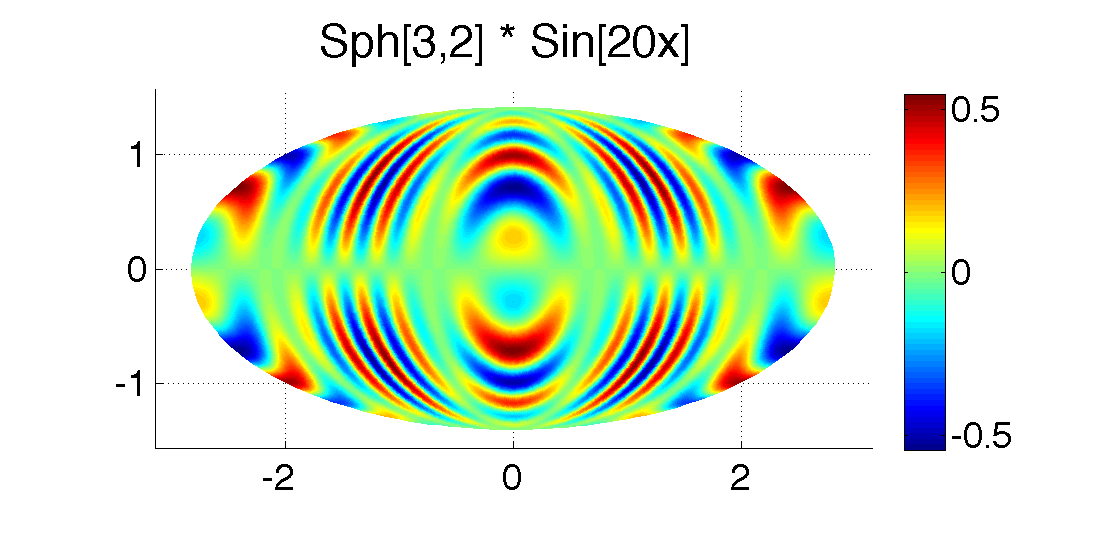
\includegraphics[width=1.0\textwidth]{../figures/appendices/direct_vs_indirect_weights/compare_weight_generation/xsfc_vs_xsfc_alt_on_sph32_times_sine_20x/sph32_times_sin20x.eps}
	\caption{Test function:  \\ $f(\vx) = Y_{3}^{2}(\vx)\sin(20x)$.  }
	\end{subfigure}
	
	\begin{subfigure}[t]{0.48\textwidth}
		\centering
	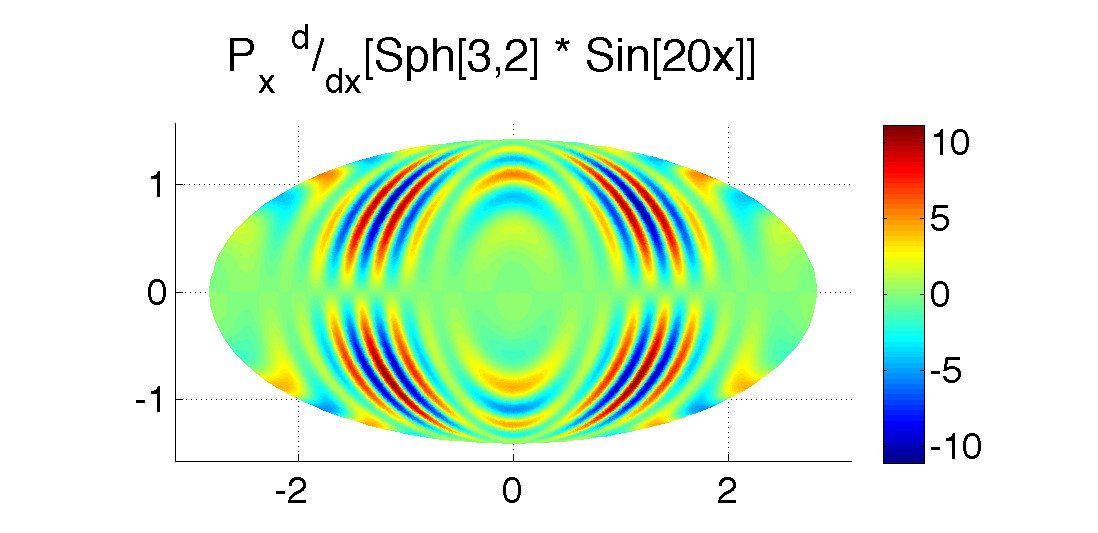
\includegraphics[width=1.0\textwidth]{../figures/appendices/direct_vs_indirect_weights/compare_weight_generation/xsfc_vs_xsfc_alt_on_sph32_times_sine_20x/pdx_sph32_times_sin20x.eps}
	\caption{Projected $x$-derivative: \\	$\mathbf{p}_{x} \cdot \nabla f(\vx)$.  }
	\end{subfigure}
	\begin{subfigure}[t]{0.48\textwidth}
		\centering
	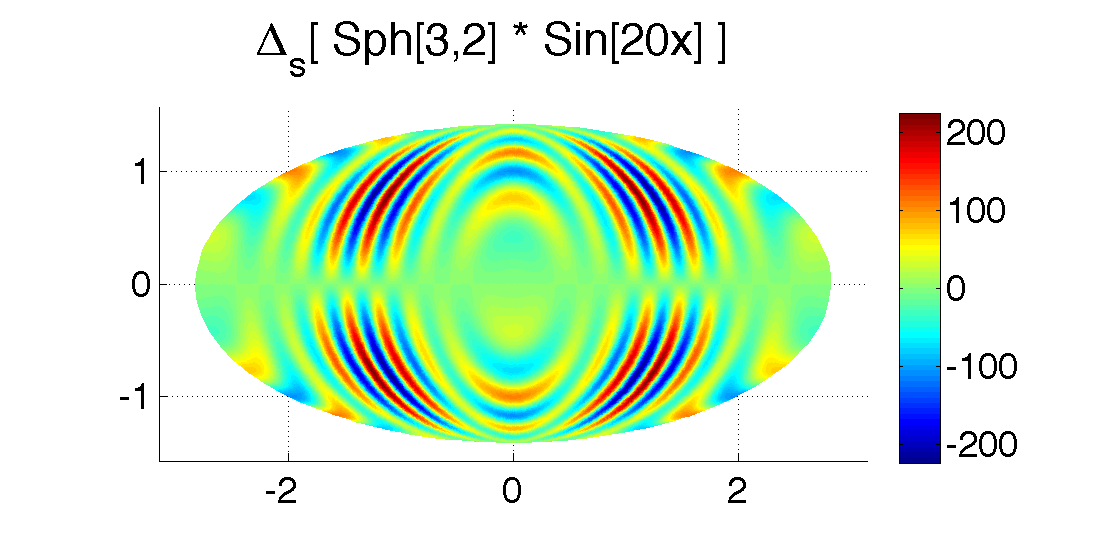
\includegraphics[width=1.0\textwidth]{../figures/appendices/direct_vs_indirect_weights/compare_weight_generation/lsfc_vs_px_grad_dot_px_grad/lsfc_sph32_times_sin20x.eps}
	\caption{Surface Laplacian: \\ $\LaplaceBeltrami f(\vx)$.  }
	\end{subfigure}
	\caption{Test function and its projected derivatives on the surface of the unit sphere. }
	\end{center}
\end{figure}

\begin{figure}
	\centering
	\begin{subfigure}[t]{0.48\textwidth}
	\includegraphics[width=1.0\textwidth]{../figures/appendices/direct_vs_indirect_weights/compare_weight_generation/xsfc_vs_xsfc_alt_on_sph32_times_sine_20x/direct_rel_l2_error.eps}
	\caption{$\mathbf{p}_{x} \cdot \nabla f(\vx)$ }
	\end{subfigure}
	\begin{subfigure}[t]{0.48\textwidth}
	\includegraphics[width=1.0\textwidth]{../figures/appendices/direct_vs_indirect_weights/compare_weight_generation/lsfc_vs_px_grad_dot_px_grad/direct_rel_l2_error.eps}
	\caption{$\LaplaceBeltrami f(\vx)$}
    \end{subfigure}
	\caption{Relative $\ell_{2}$ error in differentiation.}
\end{figure}


\begin{figure}
	\centering
	\begin{subfigure}[t]{0.48\textwidth}
	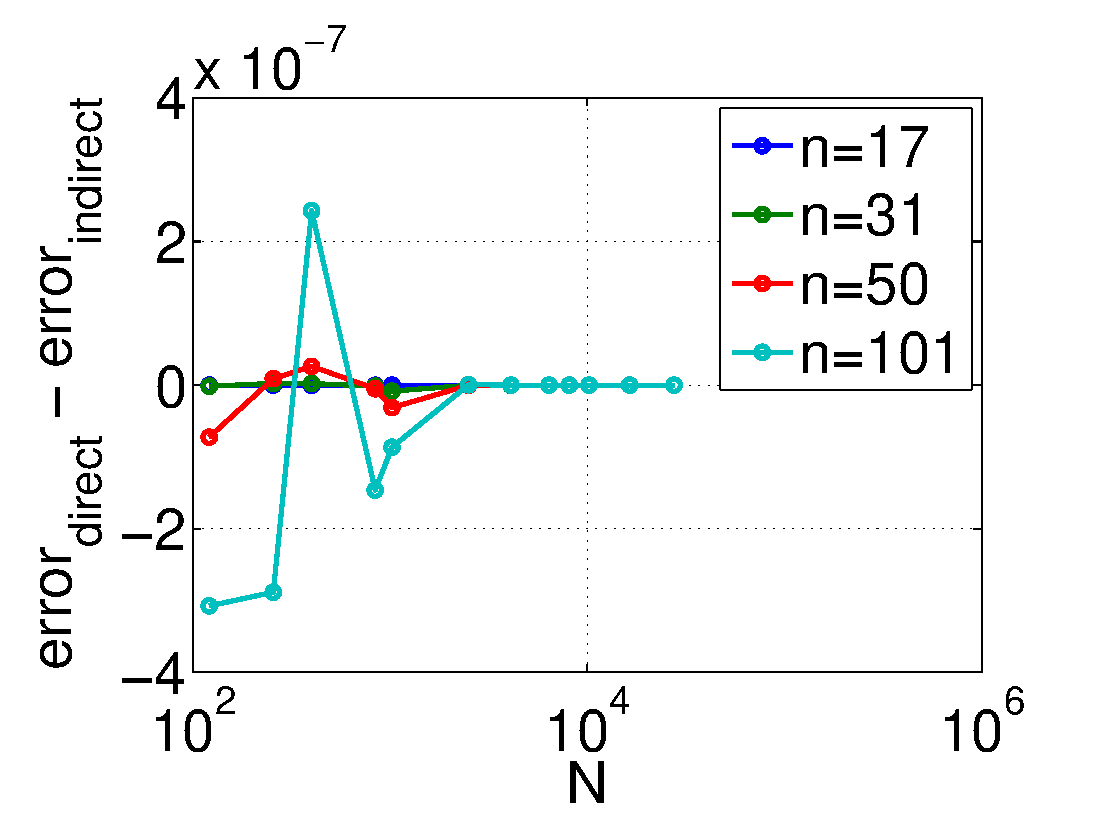
\includegraphics[width=1.0\textwidth]{../figures/appendices/direct_vs_indirect_weights/compare_weight_generation/xsfc_vs_xsfc_alt_on_sph32_times_sine_20x/diff_of_rel_l2_errors.eps}
	\caption{$\mathbf{p}_{x} \cdot \nabla ( Y_{3}^{2} \sin(20 x))$}
	\end{subfigure}
		\begin{subfigure}[t]{0.48\textwidth}
	\centering
	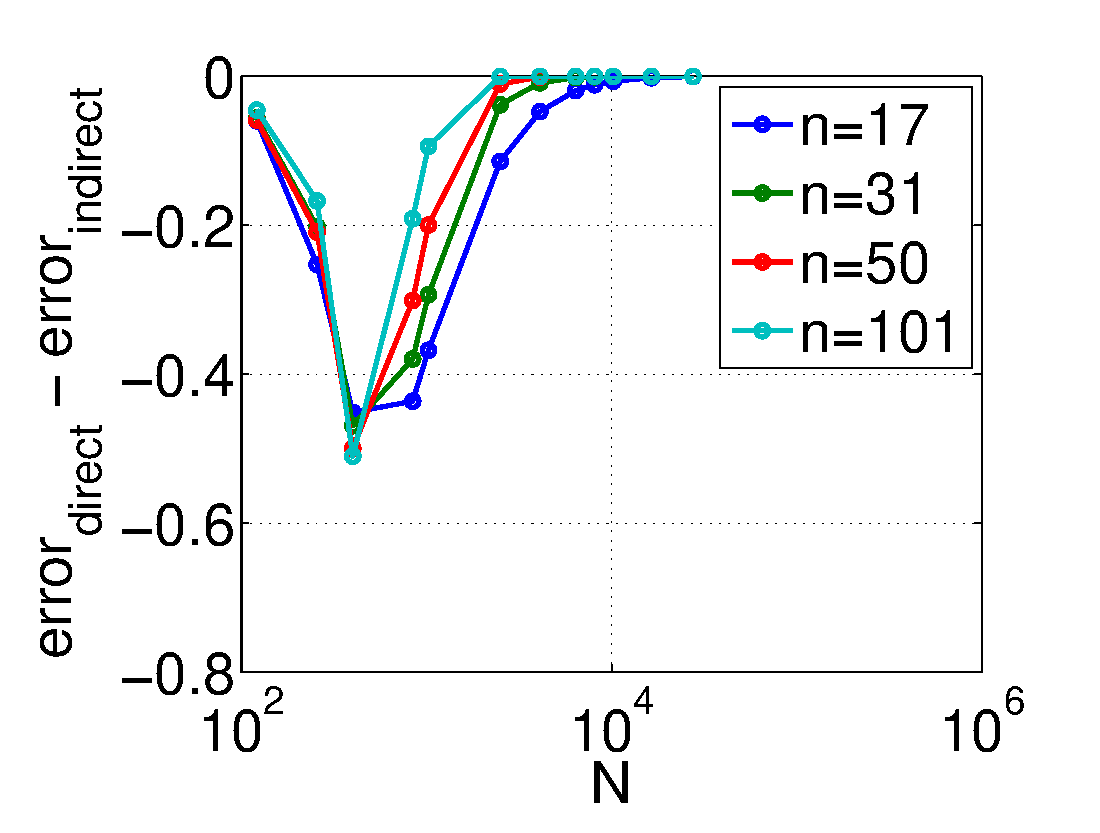
\includegraphics[width=1.0\textwidth]{../figures/appendices/direct_vs_indirect_weights/compare_weight_generation/lsfc_vs_px_grad_dot_px_grad/diff_of_rel_l2_errors.eps}
	\caption{$\LaplaceBeltrami$ of $Y_{3}^{2} \sin(20 x)$ (Indirect error is significantly higher for small resolutions. This likely due to compounding errors from the operator $P_x (D_x D_x + D_y D_y + D_z D_z)$). Where negative this figure indicates that the error is higher for indirect weight calculation. }
	\end{subfigure}
	\caption{Signed differences of relative $\ell_{2}$ errors in differentiation between Direct and Indirect weights. The sign indicates on the error indicates the higher of the two weight approaches.}
\end{figure}


\begin{figure}
	\centering
		\begin{subfigure}[t]{0.48\textwidth}
		\centering
	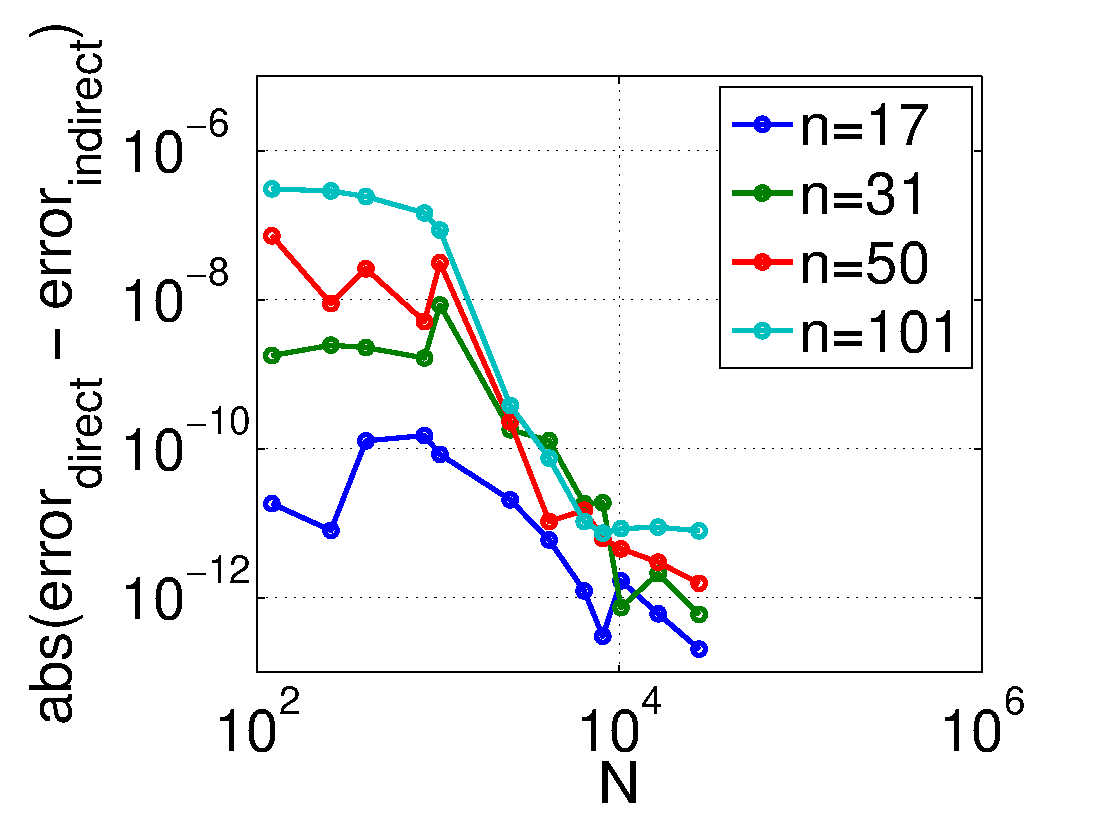
\includegraphics[width=1.0\textwidth]{../figures/appendices/direct_vs_indirect_weights/compare_weight_generation/xsfc_vs_xsfc_alt_on_sph32_times_sine_20x/abs_diff_of_rel_l2_errors.eps}
	\caption{$\mathbf{p}_{x} \cdot \nabla ( Y_{3}^{2} \sin(20 x))$}
	\end{subfigure}
	\begin{subfigure}[t]{0.48\textwidth}
	\centering
	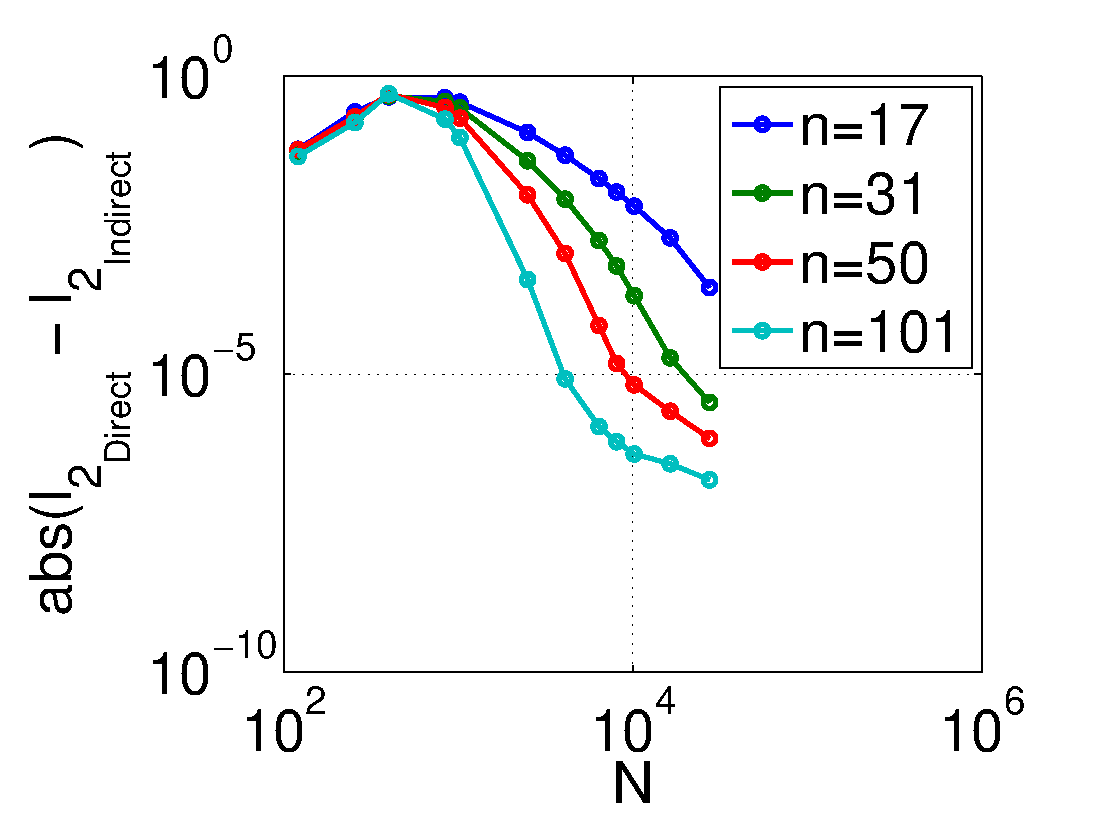
\includegraphics[width=1.0\textwidth]{../figures/appendices/direct_vs_indirect_weights/compare_weight_generation/lsfc_vs_px_grad_dot_px_grad/abs_diff_of_rel_l2_errors.eps}
	\caption{$\LaplaceBeltrami$ of $Y_{3}^{2} \sin(20 x)$}
	\end{subfigure}
		\caption{Absolute differences of relative $\ell_{2}$ errors in differentiation between Direct and Indirect weights.}
\end{figure}

%% NOT USEFUL: %%
%\begin{figure}[htbp]
%\centering
%\includegraphics[width=0.425\textwidth]{../figures/chapter2/compare_weight_generation/xsfc_vs_xsfc_alt_on_sph32/condest_dm_xsfc.pdf}
%\caption{Condition number estimates (condest) of direct $\mathbf{p}_{x}\nabla$ differentiation matrix}
%\end{figure}


\section{Conclusions}

%TODO: It appears that indirect weight calculations function. 
%TODO: They do have potential for savings
%TODO: Low resolution amplifies the errors in indirect weights. 
%TODO: still need to compare with the RBF-GA stable weight methods. What if stable weights initially resolve the extra error we see for small resolutions?




%Although it is clear the indirect method functions well compared to the direct method, we must consider its usefulness. Typically, weights are computed only as necessary for a PDE. If the PDE is on the sphere, then directly computing the $\mathbf{P}\cdot \nabla$ operator would be most efficient for both memory and computation. However, one could imagine a scenario such as a 3-D spherical shell domain with physics on the boundaries that must be constrained to the surface, while the interior requires only an unprojected $\nabla$ operator. In such cases, by simply computing for the $\nabla$ operator, we assemble all necessary operators with minimal loss of accuracy and significant savings ($3Nn$ doubles) in storage. 


%\ifstandalone
%\bibliographystyle{plain}
%\bibliography{merged_references}
%\end{document}
%\else
%\expandafter\endinput
%\fi


\ifstandalone
\bibliographystyle{plain}
\bibliography{merged_references}
\end{document}
\else
\expandafter\endinput
\fi

